\pdfbookmark{Общая характеристика работы}{characteristic}             % Закладка pdf
\section*{Общая характеристика работы}

\newcommand{\actuality}{\pdfbookmark[1]{Актуальность}{actuality}\underline{\textbf{\actualityTXT}}}
\newcommand{\progress}{\pdfbookmark[1]{Разработанность темы}{progress}\underline{\textbf{\progressTXT}}}
\newcommand{\aim}{\pdfbookmark[1]{Цели}{aim}\underline{{\textbf\aimTXT}}}
\newcommand{\tasks}{\pdfbookmark[1]{Задачи}{tasks}\underline{\textbf{\tasksTXT}}}
\newcommand{\aimtasks}{\pdfbookmark[1]{Цели и задачи}{aimtasks}\aimtasksTXT}
\newcommand{\novelty}{\pdfbookmark[1]{Научная новизна}{novelty}\underline{\textbf{\noveltyTXT}}}
\newcommand{\influence}{\pdfbookmark[1]{Практическая значимость}{influence}\underline{\textbf{\influenceTXT}}}
\newcommand{\methods}{\pdfbookmark[1]{Методология и методы исследования}{methods}\underline{\textbf{\methodsTXT}}}
\newcommand{\defpositions}{\pdfbookmark[1]{Положения, выносимые на защиту}{defpositions}\underline{\textbf{\defpositionsTXT}}}
\newcommand{\reliability}{\pdfbookmark[1]{Достоверность}{reliability}\underline{\textbf{\reliabilityTXT}}}
\newcommand{\probation}{\pdfbookmark[1]{Апробация}{probation}\underline{\textbf{\probationTXT}}}
\newcommand{\contribution}{\pdfbookmark[1]{Личный вклад}{contribution}\underline{\textbf{\contributionTXT}}}
\newcommand{\publications}{\pdfbookmark[1]{Публикации}{publications}\underline{\textbf{\publicationsTXT}}}


{\actuality} Современные интернет-сети становятся все более сложными, а также характеризуются высокой динамичностью изменений, что предъявляет высокие требования к методам их анализа и оценке производительности в режиме реального времени или близким к таковым по скорости. Эффективность работы сети напрямую зависит от множества факторов, включая нагрузку на каналы передачи данных, количество активных пользователей, процесс маршрутизации, а также используемые типы устройств. Все это влияет на качество обслуживания (QoS - Quality-of-Service) в условиях ограниченного вычислительного ресурса. С увеличением объема данных и числа подключенных устройств требуется разработка новых подходов для мониторинга и анализа работы сетей в реальном времени.

Однако в условиях ограниченного вычислительного ресурса, а также необходимости обеспечения быстродействия и масштабируемости, использование сложных моделей машинного обучения, таких как глубокие нейронные сети, оказывается не всегда оправданным. Эти модели требуют значительных вычислительных мощностей и памяти, что усложняет процесс внедрения в реальных системах с ограниченными ресурсами. Многие современные исследования указывают на необходимость в поиске альтернатив для задач сетевого мониторинга, в частности при применении устройств периферии сети (edge device) \cite{Xu2019LightweightNet, Wang2024Lightweight, Liu2022Analysis}. Также стоит подчеркнуть, что различные ресурсоемкие методы (в частности нейросетевые подходы) требуют больших серверных мощностей, а значит необходима передача данных с точки сбора до данного сервера, что может не проходить по ограничениям по времени, а также нарушать требования безопасности при транспортировке чувствительных данных. В связи с перечисленными проблемами требуется разработка и применение легковесных алгоритмов, которые позволяют на должном уровне точности анализировать производительность интернет-сетей при минимальных затратах ресурсов и таким образом не теряя свою эффективность с ростом сетевой инфраструктуры и увеличением количества пользователей.


%\textbf{Актуальность работы}

%\textbf{Степень разработанности темы}
%(Есть множество публикаций по теме, но в них идет фокус на использовании DNN, что значительно отличается от вектора данной работы. )

{\aim} данной работы является исследование и разработка методологии анализа записей сетевого трафика, методов прогнозирования времени отклика узлов сети для применения на периферийных сетевых устройствах с высокой вычислительной нагрузкой.

%данной работы является исследование и разработка методов обработки и анализа интернет-трафика и данных интернет-сетей, в частности анализ доступности соединения, с упором на использование легковесных методов и алгоритмов, в частности относящихся к технологиям TinyML.


Для достижения данной цели были поставлены следующие {\tasks}:
\begin{enumerate}[beginpenalty=10000] 
	\item Исследовать записи сетевого трафика из открытых источников,  провести сравнительный анализ методов \phantom{ } генерации \phantom{ } и преобразования признаков, провести разработку моделей классификаторов трафика с учётом ограничений вычислительной сложности, сформировать признаковое пространство для повышения метрик классификации трафика.
	\item Провести исследование распределенных систем измерений параметров интернет сетей, разработать методы предобработки и калибровки получаемых показателей.
	\item Разработать методы анализа и прогнозирования времени отклика при учёте применения периферийных сетевых устройств с высокой вычислительной нагрузкой. 
	%\item Провести исследование современных решений задачи анализа интернет-сетей, в частотности в условиях ограничений на вычислительные мощности. 
	%\item Исследовать данные о трафике из открытых источников и провести апробацию и сравнение методов анализа соединений, применяемых с целью обеспечения необходимого уровня QoS.
	%\item Провести сбор и исследование данных о состоянии сетевой инфраструктуры. Разработать методы предобработки полученных данных.
	%\item Разработать методы анализа и оценки состояния компьютерных сетей, в том числе в режиме реального времени. При ведении разработки учитывать малую мощность применяемых устройств: отказ от использования глубоких нейронных сетей (DNN) и высоконагруженных ансамблевых методов машинного обучения.  
	%\item \ldots
\end{enumerate}


%{\novelty}
%\begin{enumerate}[beginpenalty=10000] 
%	\item Предложен комплексный набор методов предобработки и калибровки получаемых показателей \ldots
%	\item Разработана система оценки загруженности сети, не использующая прямых измерений. \ldots%
%	\item Было выполнено оригинальное исследование на реальных данных работы сети на территории РФ, формирующее актуальную картину работы сетей\ldots
%	\item ...
%\end{enumerate}

{\defpositions}
\begin{enumerate}[beginpenalty=10000]
	\item Проведенный разведочный анализ, исследование и разработка методологии анализа данных сетевого домена позволили выявить ковариационный сдвиг в ряде датасетов и улучшить модели классификации (увеличение accuracy не менее чем на 0,2), а также выявить оптимальные методы предобработки.
	
	\item Анализ и исследование особенностей программно-аппаратных платформ системы RIPE Atlas привел к разработке методов предобработки и калибровки получаемых данных, которые позволяют компенсировать временную задержку у 63\% устройств, обеспечивая их функциональную эквивалентность 37\% эталонных устройств и совместимость с едиными аналитическими методами.
	
	\item Разработанные и исследованные алгоритмы динамической кластеризации измерительных зондов по показателям времени отклика на территории РФ с применением методов машинного обучения позволили выделить 32\% аномальных узлов, фильтрация которых привела к снижению ошибки (RMSE) прогнозирования времени приема-передачи до 50\%.
	
	\item Разработанные и исследованные алгоритмы прогнозирования времени приема-передачи (round-trip-time, RTT) в детектируемых кластерах измерительных зондов позволили использовать на 3 порядка меньше операций с плавающей запятой (FLOPs) при достижении сопоставимой точности в сравнении с передовыми нейросетевыми подходами.
	
\end{enumerate}

%\textbf{Практическая значимость/Теоретическая значимость}


{\reliability} \phantom{ } полученных результатов \phantom{ } обеспечивается использованием методов статистического анализа, машинного обучения, математическим моделированием, совпадением результатов исследования с экспериментальными данными, а также непосредственным участием автора в получении исходных данных и проведении экспериментов.


\textbf{Апробация работы.} Основные результаты работы докладывались на
следующих научных конференциях:
	\begin{enumerate}[beginpenalty=10000]
		\item VI международная конференция
		«Информационные технологии и технические средства управления» (ICCT-2022), Институт проблем
		управлений им. В.А.Трапезникова РАН совместно с Астраханским государственным
		техническим университетом, 2022 г.
		\item X Международная конференция  «Инжиниринг  \& \\ Телекоммуникации − En\&T-2023» МФТИ, Долгопрудный
		\item 65-й Всероссийская научная конференция
		МФТИ в честь 115-летия Л.Д. Ландау 2023, МФТИ, Долгопрудный
		\item XXVI Международная конференция
		«Цифровая обработка сигналов и ее применение — DSPA-2024», Институт проблем управления им. В.А.Трапезникова РАН, Москва, Россия.
		\item XI Международная конференция  «Инжиниринг \& \\ Телекоммуникации — En\&T-2024» МФТИ, Москва.
	\end{enumerate}
	
{\publications} Основные результаты по теме диссертации изложены в 6 печатных работах, 1 из которых издана в журналах, рекомендованных ВАК, 2 –
в рецензируемых изданиях, входящих в базу данных Scopus, 3 - в тезисах докладов. Получено 1 свидетельство о регистрации программы для ЭВМ.




 % Характеристика работы по структуре во введении и в автореферате не отличается (ГОСТ Р 7.0.11, пункты 5.3.1 и 9.2.1), потому её загружаем из одного и того же внешнего файла, предварительно задав форму выделения некоторым параметрам

%Диссертационная работа была выполнена при поддержке грантов \dots

%\underline{\textbf{Объем и структура работы.}} Диссертация состоит из~введения,
%четырех глав, заключения и~приложения. Полный объем диссертации
%\textbf{ХХХ}~страниц текста с~\textbf{ХХ}~рисунками и~5~таблицами. Список
%литературы содержит \textbf{ХХX}~наименование.

\pdfbookmark{Содержание работы}{description}                          % Закладка pdf
\section*{Содержание работы}

Во \underline{\textbf{введении}} обосновывается актуальность исследования, проводимого в рамках данной диссертационной работы,
приводится обзор научной литературы по изучаемой проблеме анализа сетей и интернет-трафика, формулируется цель, ставятся задачи для ее достижения, излагается научная новизна, практическая значимость, а также сведения об апробации описываемой работы. В последующих главах сначала представлен обзор существующих решений по  тематике работы, затем описываются результаты анализа полученных сетевых данных и итоги применения на них разработанных методов и подходов.


\underline{\textbf{Первая глава}} посвящена общей актуализации проблемы анализа сетей и обзору современных методов анализа интернет-трафика и сетевой инфраструктуры. Описываются основные факторы, обостряющие проблему мониторинга сетей как такового в настоящее время. Также представлен сравнительный анализ как классических методов анализа трафика и сетей, так и направления в разработке альтернативных подходов, в частности использование ML и DL подходов.


\underline{\textbf{Раздел 1.1}} посвящен общей актуализации проблемы анализа сетей и обзору современных методов анализа интернет-трафика и сетевой инфраструктуры. Описываются основные факторы, обостряющие проблему мониторинга сетей и трафика как такового в настоящее время. В частности описываются общий рост мировых объемов трафика (Рисунок \ref{fig:traffic_growth}), рост использования протоколов шифрования и рост разнообразия используемых устройств.
Эти факторы приводят к уменьшению эффективности традиционных методов, на что указывают различные современные обзорные публикации. В связи с этим возникает необходимость в разработке альтернативных методов и инструментов, основанных на машинном обучении и статистическом анализе, которые являются перспективными и развивающимися. %\cite{dpi1, dpi2}


\begin{figure}[ht]
	
	\centerfloat{
		
\includegraphics[width=\textwidth]{traffic_growth}
	}
	\caption{Средний и пиковый объемы трафика во Франкфурте в период с 2018 по 2022 год}\label{fig:traffic_growth}
\end{figure}


\underline{\textbf{В разделе 1.2}} приведен обзор и сравнение классических методов анализа сетевого трафика и разрабатываемых подходов, основанных на машинном обучении и нейронных сетях. В последние годы наблюдается рост интереса к глубоким нейронным сетям (DNN) в различных сферах науки и анализ трафика не является исключением. Их главное преимущество — автоматическое извлечение признаков, однако они требуют ресурсоёмкой настройки архитектуры и высоких вычислительных затрат. Несмотря на это, DNN часто обеспечивают высокую точность, %\cite{Liu2019}
особенно с учётом современных аппаратных улучшений применяемых вычислительных мощностей.

Тем не менее, DNN не всегда применимы в условиях ограниченных вычислительных ресурсов, например, на маршрутизаторах и одноплатных устройствах. Рост объёма и шифрования интернет-трафика делает традиционные методы анализа, такие как DPI, менее эффективными. В таких условиях классические алгоритмы машинного обучения, хоть и уступают в точности, могут быть предпочтительны из-за своей меньшей вычислительной сложности. % \cite{Athanasios2019, Xiao2018}.%\cite{Sherry2015, decix}.

Deep Packet Inspection (DPI) остаётся важной технологией, применяемой для анализа содержимого пакетов и обнаружения угроз. % \cite{Chaudhary2011, Shubbar2017}. 
DPI сопоставляет входящий трафик с базой сигнатур атак и может выявлять специфичные паттерны вредоносных программ. %\cite{Lin2014} 
%(Рисунок \ref{fig:dpi1}).

Однако DPI сталкивается с рядом ограничений и проблем: широкое использование шифрования, которое затрудняет доступ к полезной нагрузке пакетов; применение нестандартных портов и маскировка протоколов; полиморфные вредоносные программы, изменяющие сигнатуры и обходящие стандартные шаблоны; высокая вычислительная нагрузка ограничивает применение DPI в реальном времени; растущий объём сетевых данных усложняют эффективный анализ; DPI вызывает опасения у пользователей по поводу конфиденциальности; применение ИИ злоумышленниками требует более интеллектуальных методов защиты.


\begin{comment}
	\begin{itemize}
		\item Широкое использование шифрования (например, TLS) затрудняет доступ к полезной нагрузке пакетов; %\cite{Ji2024};
		\item Применение нестандартных портов и маскировка протоколов снижают точность анализа; % \cite{Hou2020};
		\item Полиморфные вредоносные программы изменяют сигнатуры и обходят стандартные шаблоны;% \cite{Xue2024};
		\item Высокая вычислительная нагрузка ограничивает применение DPI в реальном времени; % \cite{Nam2022};
		\item Растущие объёмы сетевых данных усложняют эффективный анализ; %\cite{Jiang2021};
		\item DPI вызывает опасения по поводу конфиденциальности пользователей; % \cite{Barut2023};
		\item Применение \phantom{ } ИИ \phantom{ } злоумышленниками требует более интеллектуальных методов защиты; % \cite{Roshan2024}.
	\end{itemize}
\end{comment}

В ответ на эти вызовы возрастает интерес к использованию машинного обучения для анализа зашифрованного трафика без необходимости его расшифровки. %\cite{Shen2023}.

\begin{comment}
	\begin{figure}[ht]
		\centerfloat{
			
\includegraphics[scale=0.9]{intro/DPI1}
		}
		\caption{Блок-схема этапов работы метода Deep Packet Inspection (DPI)}\label{fig:dpi1}
	\end{figure}
\end{comment}



\underline{\textbf{В разделе 1.3}} рассматриваются существующие решения и проблемы задачи анализа сетевой инфраструктуры, ее эффективности и поиска проблемных участков.


Анализ производительности современных компьютерных сетей сталкивается с рядом проблем, особенно при выявлении узких мест, так называемых «бутылочных горлышек» — компонентов, ограничивающих пропускную способность (см. рисунок \ref{fig:bottleneck}). Традиционные методы, включая протокол SNMP (Simple Network Management Protocol), пороговые правила и сетевую томографию, становятся всё менее эффективными в условиях роста объёмов данных, усложнения архитектур и появления IoT-устройств. %\cite{snmp1, mlmon1}. О
ни требуют ручной настройки, плохо адаптируются к изменяющемуся трафику и не обеспечивают полной видимости картины.

\begin{figure}[ht]
	\centerfloat{
		
\includegraphics[width=0.7\textwidth]{bottleneck}
	}
	\caption{Условное изображение проблемы <<бутылочного горлышка>> в структуре компьютерных сетей }\label{fig:bottleneck} % \cite{bottleneck}
\end{figure}

Методы машинного обучения предлагают более адаптивный подход. Классические модели, такие как SVM, деревья решений и нейронные сети, позволяют обнаруживать аномалии, прогнозировать загрузку и выявлять проблемные участки без вручную настраиваемых порогов. Они успешно применяются как в центрах обработки данных, так и в распределённых средах. Глубокое обучение (DL) с применением CNN, RNN и LSTM улучшают эту способность, извлекая сложные зависимости напрямую из трафика и временных рядов. %\cite{El_Shamy2021Anomaly}   %\cite{Abbasi2021}.

Тем не менее, методы DL имеют высокие вычислительные требования, что ограничивает их использование на маломощных устройствах, особенно в IoT-сетях. 
%Здесь необходимы более быстродейственные протоколы (например, LwM2M или CoMI) и энергоэффективная аналитика. Даже классические ML-модели требуют регулярного обновления и настройки, особенно при работе с изменяющейся нагрузкой. %\cite{Jebur2025}.

Гибридные подходы, сочетающие лёгкий ML на периферии и более сложный анализ в центре, показывают хорошие результаты. Такие системы способны обеспечивать как предиктивное оповещение, так и выявление первопричин. Продолжающееся развитие графовых нейронных сетей и встроенной телеметрии делает перспективу полной автоматизации мониторинга всё более реальной. %\cite{Wang2021Empirical}.

Таким образом, традиционные подходы уже не справляются с задачами современного мониторинга. Машинное обучение предлагает более гибкие и точные инструменты, хотя их реализация требует учёта ограничений устройств и сетевой инфраструктуры. Исследования в этой области направлены на создание масштабируемых, лёгких и адаптивных решений. Итоги проведенного анализа приведены в таблице \ref{tab:methods1}.


\begin{table}[htbp]
	\centering
	\caption{Сравнение подходов к способам мониторинга сетей}
	\label{tab:methods1}
	\begin{tabular}{|>{\centering\arraybackslash}p{2.28cm}|>{\centering\arraybackslash}p{3.05cm}|>{\centering\arraybackslash}p{2.23cm}|>{\centering\arraybackslash}p{2.68cm}|}
		\hline
		\textbf{Подход}  & \textbf{Вычислительная сложность} & \textbf{Точность в комплексных сценариях} & \textbf{IoT и граничные вычисления}  \\ \hline
		Традиционный (SNMP, пороговые правила, выборка потоков)  & Низкая нагрузка (простые опросы/ пороговые правила). & Приемлемая для известных проблем, но плохая  для новых или сложных аномалий. & Хорошо подходит для высокоуровневого мониторинга (серверы, ЦОД), плохо для IoT (из-за стоимости опроса). \\ \hline
		Классический ML(SVM, decision tree, k-NN, и т.д.) & Средняя (для обучения требуется ЦП; малая нагрузка инференса) & Хорошая во многих случаях - значительно лучше, чем статические правила & Умеренно эффективно (может выполняться в облаке или на пограничных шлюзах). \\ \hline 
		Глубокое обучение(CNN, RNN, DNN и т.д.) & Высокая (крупные модели, рекомендуется использование GPU/TPU; высокая нагрузка на оборудование). & Отлично работает с большими и сложными наборами данных. & Плохо подходит для маломощных устройств Технологии TinyML могут помочь.  \\ \hline
	\end{tabular}
	
\end{table}



\underline{\textbf{Во второй главе}} описываются результаты исследования данных интернет-трафика, предоставляемых исследователями из  Канадского Института Кибербезопасности (Canadian Institute for Cybersecurity - CIC). Приведены основные результаты по применению методов генерации признаков с целью повышения метрик качества моделей машинного обучения.

\underline{\textbf{В разделе 2.1}} приведено описание использованных в работе наборов данных от CIC. 

Одной из ключевых задач анализа трафика является его классификация по типу соединения и содержимому. Среди популярных наборов данных выделяются: ISCXVPN (2016), ISCXTor2016 и CCCS-CIC-AndMal (2020), разработанные Канадским институтом кибербезопасности (CIC).

\textbf{ISCXVPN (2016)} позволяет проводить сравнительный анализ VPN и не-VPN трафика. Признаки включают такие величины как среднее число пакетов в секунду, 
длительность соединения, битрейт, а также различные статистики по направлениям от и до адресата. В наборе данных охватываются различные типы соединений: HTTP/HTTPS, общение в чатах, email, стриминг, FTP, VoIP, P2P.


\begin{comment}
	\begin{itemize}
		\item Среднее число пакетов в секунду
		\item Пропускная способность
		\item Длительность соединения
		\item Статистики по направлениям от и до адресата (среднее, максимум и т.д.)
	\end{itemize}
\end{comment}

\textbf{ISCXTor2016} — содержит данные о трафике через сеть Tor и открытое соединение. В качестве ключевой проблемы стоит отметить сильный дисбаланс классов (рисунок \ref{fig:tor_balance}).


\begin{figure}[ht]
	\centering
	\begin{minipage}[t]{0.49\textwidth}
		\centering
		
\includegraphics[scale=0.35]{CIC/vpn_balance}
		\caption{Баланс VPN и не-VPN трафика в ISCXVPN (2016)}
		\label{fig:vpn_balance}
	\end{minipage}
	\hfill
	\begin{minipage}[t]{0.49\textwidth}
		\centering
		
\includegraphics[scale=0.58]{CIC/tor_balance}
		\caption{Баланс Tor и не-Tor трафика в ISCXTor2016} 
		\label{fig:tor_balance}
	\end{minipage}

\end{figure}



\textbf{CCCS-CIC-AndMal (2020)} — классификация Android-программ: 200K вредоносных и 200K легитимных. Вредоносное ПО разбито на 14 категорий и 191 семейств. В этом наборе данных также отмечается дисбаланс по классам, а именно по упомянутым категориям и семейств вредоносных программ.

\begin{comment}
	\begin{table}[htbp]
		\centering
		\caption{Количественное описание изучаемых данных по категориям вредоносных программ}
		\begin{tabular}{|>{\centering}p{3.8cm}|c|>{\centering\arraybackslash}p{2cm}|}  
			\hline
			\textbf{Категория} & \textbf{Количество семейств} & \textbf{Количество образцов}                    \\ \hline
			Рекламоносители (Adware)                    & 48                       & 47\,210                     \\ \hline
			Бэкдор (Backdoor)                           & 11                       & 1\,538                      \\ \hline
			Программы-вымогатели (Ransomware)           & 8                        & 6\,202                      \\ \hline
			Троян (Trojan)                              & 45                       & 13\,559                     \\ \hline
			Троян-Банкир (Trojan-Banker)                & 11                       & 887                        \\ \hline
			Троян-Дроппер (Trojan-Dropper)              & 9                        & 2\,302                      \\ \hline
			Троян-SMS (Trojan-SMS)                      & 11                       & 3\,125                      \\ \hline
			Тролян-Шпион (Trojan-Spy)                   & 11					   & 3\,540				        \\ \hline
			Вирус нулевого дня (Zero-Day)               & -                        & 13\,340                     \\ \hline
			Файловый вирус (FileInfector)			    & 5     				   & 669 						\\ \hline
			Потенциально нежелательное приложение (PUA) & 8     				   & 6\,202					    \\ \hline
			ПО с потенциальным риском (Riskware)		& 21   					   & 97\,349  					\\ \hline
			Пугающее ПО (Scareware)						& 3    					   & 1\,556						\\ \hline
			Без категории				      			& -						   & 2\,296 						\\ \hline
		\end{tabular}
		\label{tab:malware_families}
	\end{table}
	
\end{comment}



%Эти наборы используются для обучения и тестирования различных ML и DL моделей. Чаще всего используемые метрики: accuracy (точность), precision (точность), recall (полнота) и F1-метрика (F1-score). Однако следует отметить, что метрика accuracy обладает существенным ограничением: её репрезентативность существенно снижается в условиях несбалансированности классов.

%Анализ современных научных публикаций по теме анализа трафика (в том числе с применением описанных наборов данных) показывают, что методы \textbf{DPI/DFI} — становятся все менее эффективны, особенно с ростом шифрования. В то же время алгоритмы классического машинного обучения широко используются для анализа трафика и позволяют достичь метрики accuracy (точности) плоть до 95\%. Нейросетевые модели позволяют автоматически извлекать признаки и достигать высоких показателей целевых метрик. А \textbf{эволюционные алгоритмы}, \textbf{LDA}, \textbf{PCA}, а также \textbf{методы ранжирования признаков} — значимо улучшают эффективность моделей и позволяют достичь accuracy до 98-99,8 \%. %\cite{Saber2019, Haitham2019}.

\begin{comment}
	\begin{itemize}
		\item Методы \textbf{DPI/DFI} — становятся все менее эффективны, особенно с ростом шифрования. %\cite{Bregni2010}.
		\item Классическое машинное обучение, такие как \textbf{Наивный байес}, \textbf{SVM} и \textbf{WKNN} — широко используются для анализа трафика и позволяют достичь метрики accuracy (точности) плоть до 95\%.
		\item \textbf{Автоэнкодеры}, \phantom{ }\textbf{CNN}, \phantom{ }\textbf{DBN}, \phantom{ }\textbf{LSTM} — позволяют автоматически извлекать признаки и достигать высоких показателей целевых метрик %\cite{Haitham2019, Yuan2014, Hou2016, Nix2019}
		\item \textbf{Эволюционные алгоритмы}, \textbf{LDA}, \textbf{PCA}, а также \textbf{методы ранжирования признаков} — значимо улучшают эффективность моделей и позволяют достичь accuracy до 98-99,8 \% %\cite{Saber2019, Haitham2019}.
	\end{itemize}
\end{comment}


%Таким образом, можно подчеркнуть, что методы с использованием нейронных сетей являются довольно эффективными, но в то же время они обладают высокой вычислительной стоимостью. Классическое машинное обучение в купе с методами обработки признаков являются перспективным направлением в этом аспекте, а  представленные датасеты и методы дают обширную основу для исследования в области сетевой безопасности и обнаружения вредоносных приложений.

Далее, в \underline{\textbf{разделе 2.2} } описываются результаты применения методов генерации и обработки признаков, использованных на вышеописанных наборах данных.


В \underline{\textbf{подразделе 2.2.1}} представлены результаты применения AGMV. 


Одним из исследуемых методов генерации признаков был Accumulated Generalized Mean Value (AGMV, обобщенное накопленное среднее значение). Этот подход позволяет анализировать поведение временных рядов и выявлять переходы между классами данных. Формула AGMV определяется следующим образом:

$$
AGMV (x_j (t_i), p, a, K, M) = \left \{ \frac{1}{M-K}\sum_{i=K, i = i + a}^{M-1} (\left | x_j(t_i) \right |^{p}) \right \} ^{1/p},
$$
где $x_j$ — временной ряд на интервале [K, M], $p$ — параметр чувствительности, $a$ — шаг децимации, а $M-K$ — длина окна.

Метод AGMV применяется к блокам данных отдельно и преобразует исходные признаки в новые, более информативные. Он может работать подобно среднему арифметическому, геометрическому или гармоническому в зависимости от значения $p$. % Подробности можно найти в \cite{Ivch_2021}.

Было проведено исследование эффективности AGMV на двух наборах данных: ISCXVPN (бинарная классификация трафика) и CCCS-CIC-AndMal-2020 (мультиклассовая классификация вредоносного ПО). Для обеих задач использовались четыре модели машинного обучения: Случайный лес (Random Forest), дерево решений (Decision Tree), градиентный бустинг (XGBoost) и метод опорных векторов (SVM). AGMV применялся с параметрами: $w=400$, $a=1$, $p=1$.

На рисунке \ref{fig:vpn_best} представлены результаты бинарной классификации для лучших комбинаций гиперпараметров. Использование AGMV позволило достичь accuracy свыше 0,95 с моделью Random Forest. Аналогично, на рисунке \ref{ar_acc_best} показаны результаты мультиклассовой классификации вредоносных программ. Здесь также был достигнут уровень accuracy выше 0,95, что демонстрирует эффективность подхода.

\begin{comment}
	\begin{figure}[h]
		\center{
\includegraphics[width=6 cm]{VPN_best_estimator.png}}
		\caption{Accuracy для лучших кандидатов (комбинации гиперпараметров) для бинарной классификации с и без использования AGMV на наборе данных ISCXVPN для алгоритма случайного леса (RandomForest)}
		\label{fig:vpn_best}
	\end{figure} 
	
	\begin{figure}[h]
		\center{
\includegraphics[width=6 cm]{AR_Accuracy.png}}
		\caption{Accuracy для лучших кандидатов (комбинации гиперпараметров) для мультиклассовой классификации с и без использования AGMV на наборе данных CCCS-CIC-AndMal (Before reboot сценарий) для моделей случайного леса (RandForest), дерева решений (Tree), машины опорных векторов (SVM) и градиентного бустинга (XGB)}
		\label{ar_acc_best}
	\end{figure}
\end{comment}


\begin{figure}[ht]
	\centerfloat{
		\hfill
		\subcaptionbox{\label{fig:vpn_best}}{%
			
\includegraphics[width=0.505\linewidth]{VPN_best_estimator.png}}
		\hfill
		\subcaptionbox{\label{ar_acc_best}}{%
			
\includegraphics[width=0.475\linewidth]{AR_Accuracy.png}
			}
		\hfill
	}
	\caption{Accuracy для лучших кандидатов (комбинации гиперпараметров) с и без использования AGMV а) - Для бинарной классификации на наборе данных ISCXVPN для алгоритма случайного леса (RandomForest), б) - Для мультиклассовой классификации на наборе данных CCCS-CIC-AndMal (Before reboot сценарий) для моделей случайного леса (RandForest), дерева решений (Tree), машины опорных векторов (SVM) и градиентного бустинга (XGB)}
	%\label{fig:qt2}
\end{figure}




Таким образом, метод AGMV оказался эффективным для улучшения качества классификации, как в задаче анализа сетевого трафика, так и в задаче обнаружения вредоносного ПО. В дальнейшем планируется исследовать влияние параметров AGMV на качество классификации и расширить применение метода на другие типы данных.

В \underline{\textbf{подразделе 2.2.2}} представлены результаты применения CAPoNef. 


Еще одним исследуемым методом генерации признаков был метод CAPoNef. Его принцип несколько отличается от рассматриваемого ранее AGMV.
CAPoNeF (Comparative Analysis of the Positive and Negative Fluctuations) - это метод, который производит анализ временных рядов, но его отличительной особенностью является то, что ряды в нем анализируются как бестрендовоые последовательности (trendless sequences (TLS)).

Суть метода заключается в извлечении признаков из временных последовательностей, при условии, что они являются бестрендовыми, то есть в них нет значимого роста или падения среднего значения наблюдаемой величины. Метод включает в себя среднее значение, но главное - ряд характеристик для отклонений значений ряда от среднего значения, таких как диапазон между положительными и отрицательными флуктуациями, баланс между ними, размах их значений и другие, связанные с ними величины. Метод применялся как к характеристикам исходящих, так и входящих сообщений и пакетов (рисунок \ref{fig:caponefgeneral}). В итоге для каждого меняющегося во времени параметра было получено 7 новых признаков.

\begin{figure}[ht]
	\centering
	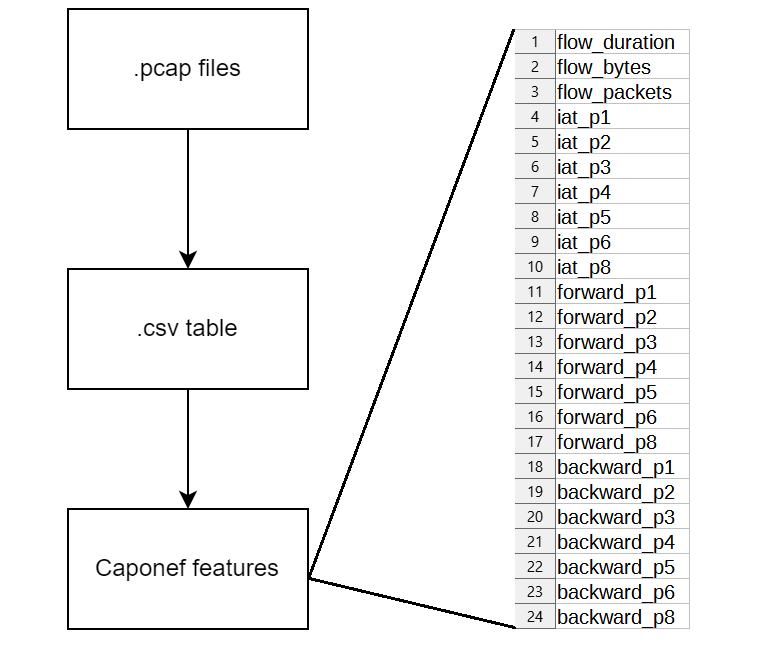
\includegraphics[width=0.7\linewidth]{images/caponef/caponef}
	\caption{Схема генерации признаков из исходных файлов}
	\label{fig:caponefgeneral}
\end{figure}

Метод был разработан в МФТИ и был впервые освящен в 2020 году. Данный метод уже показал свою эффективность в работах посвященных радиометрической идентификации, а также для задачи анализа уровня сахара в крови. % \cite{Nigmatullin2020, Nigmatullin2021}.

В работе сравнивались два набора признаков для задачи бинарной классификации VPN/non-VPN трафика: исходный набор из 4 метрик для каждой величины (среднее, стандартное отклонение, минимум и максимум интервалов между прибытием пакетов — IAT; метрики от авторов набора данных), пересчитанный из исходных .pcap-файлов, и расширенный набор из 7 метрик, полученных с использованием метода CAPoNeF. На этих данных обучались модели случайного леса (scikit-learn) и градиентного бустинга (XGBoost); максимальная достигнутая точность (accuracy) составила 0,8 при анализе 15-секундных фрагментов соединений (рисунок \ref{fig:capo}). Несмотря на увеличение размерности признакового пространства, CAPoNeF не продемонстрировал значимого улучшения качества классификации по сравнению с базовым набором, что указывает на его неэффективность именно для данной задачи и структуры данных. Тем не менее, метод остаётся потенциально применимым для других задач анализа трафика или наборов данных с иной структурой, что предполагает необходимость дальнейших исследований, а также смещения фокуса на альтернативные подходы к извлечению признаков для повышения точности классификации.

\begin{figure}[ht]
	\centering
	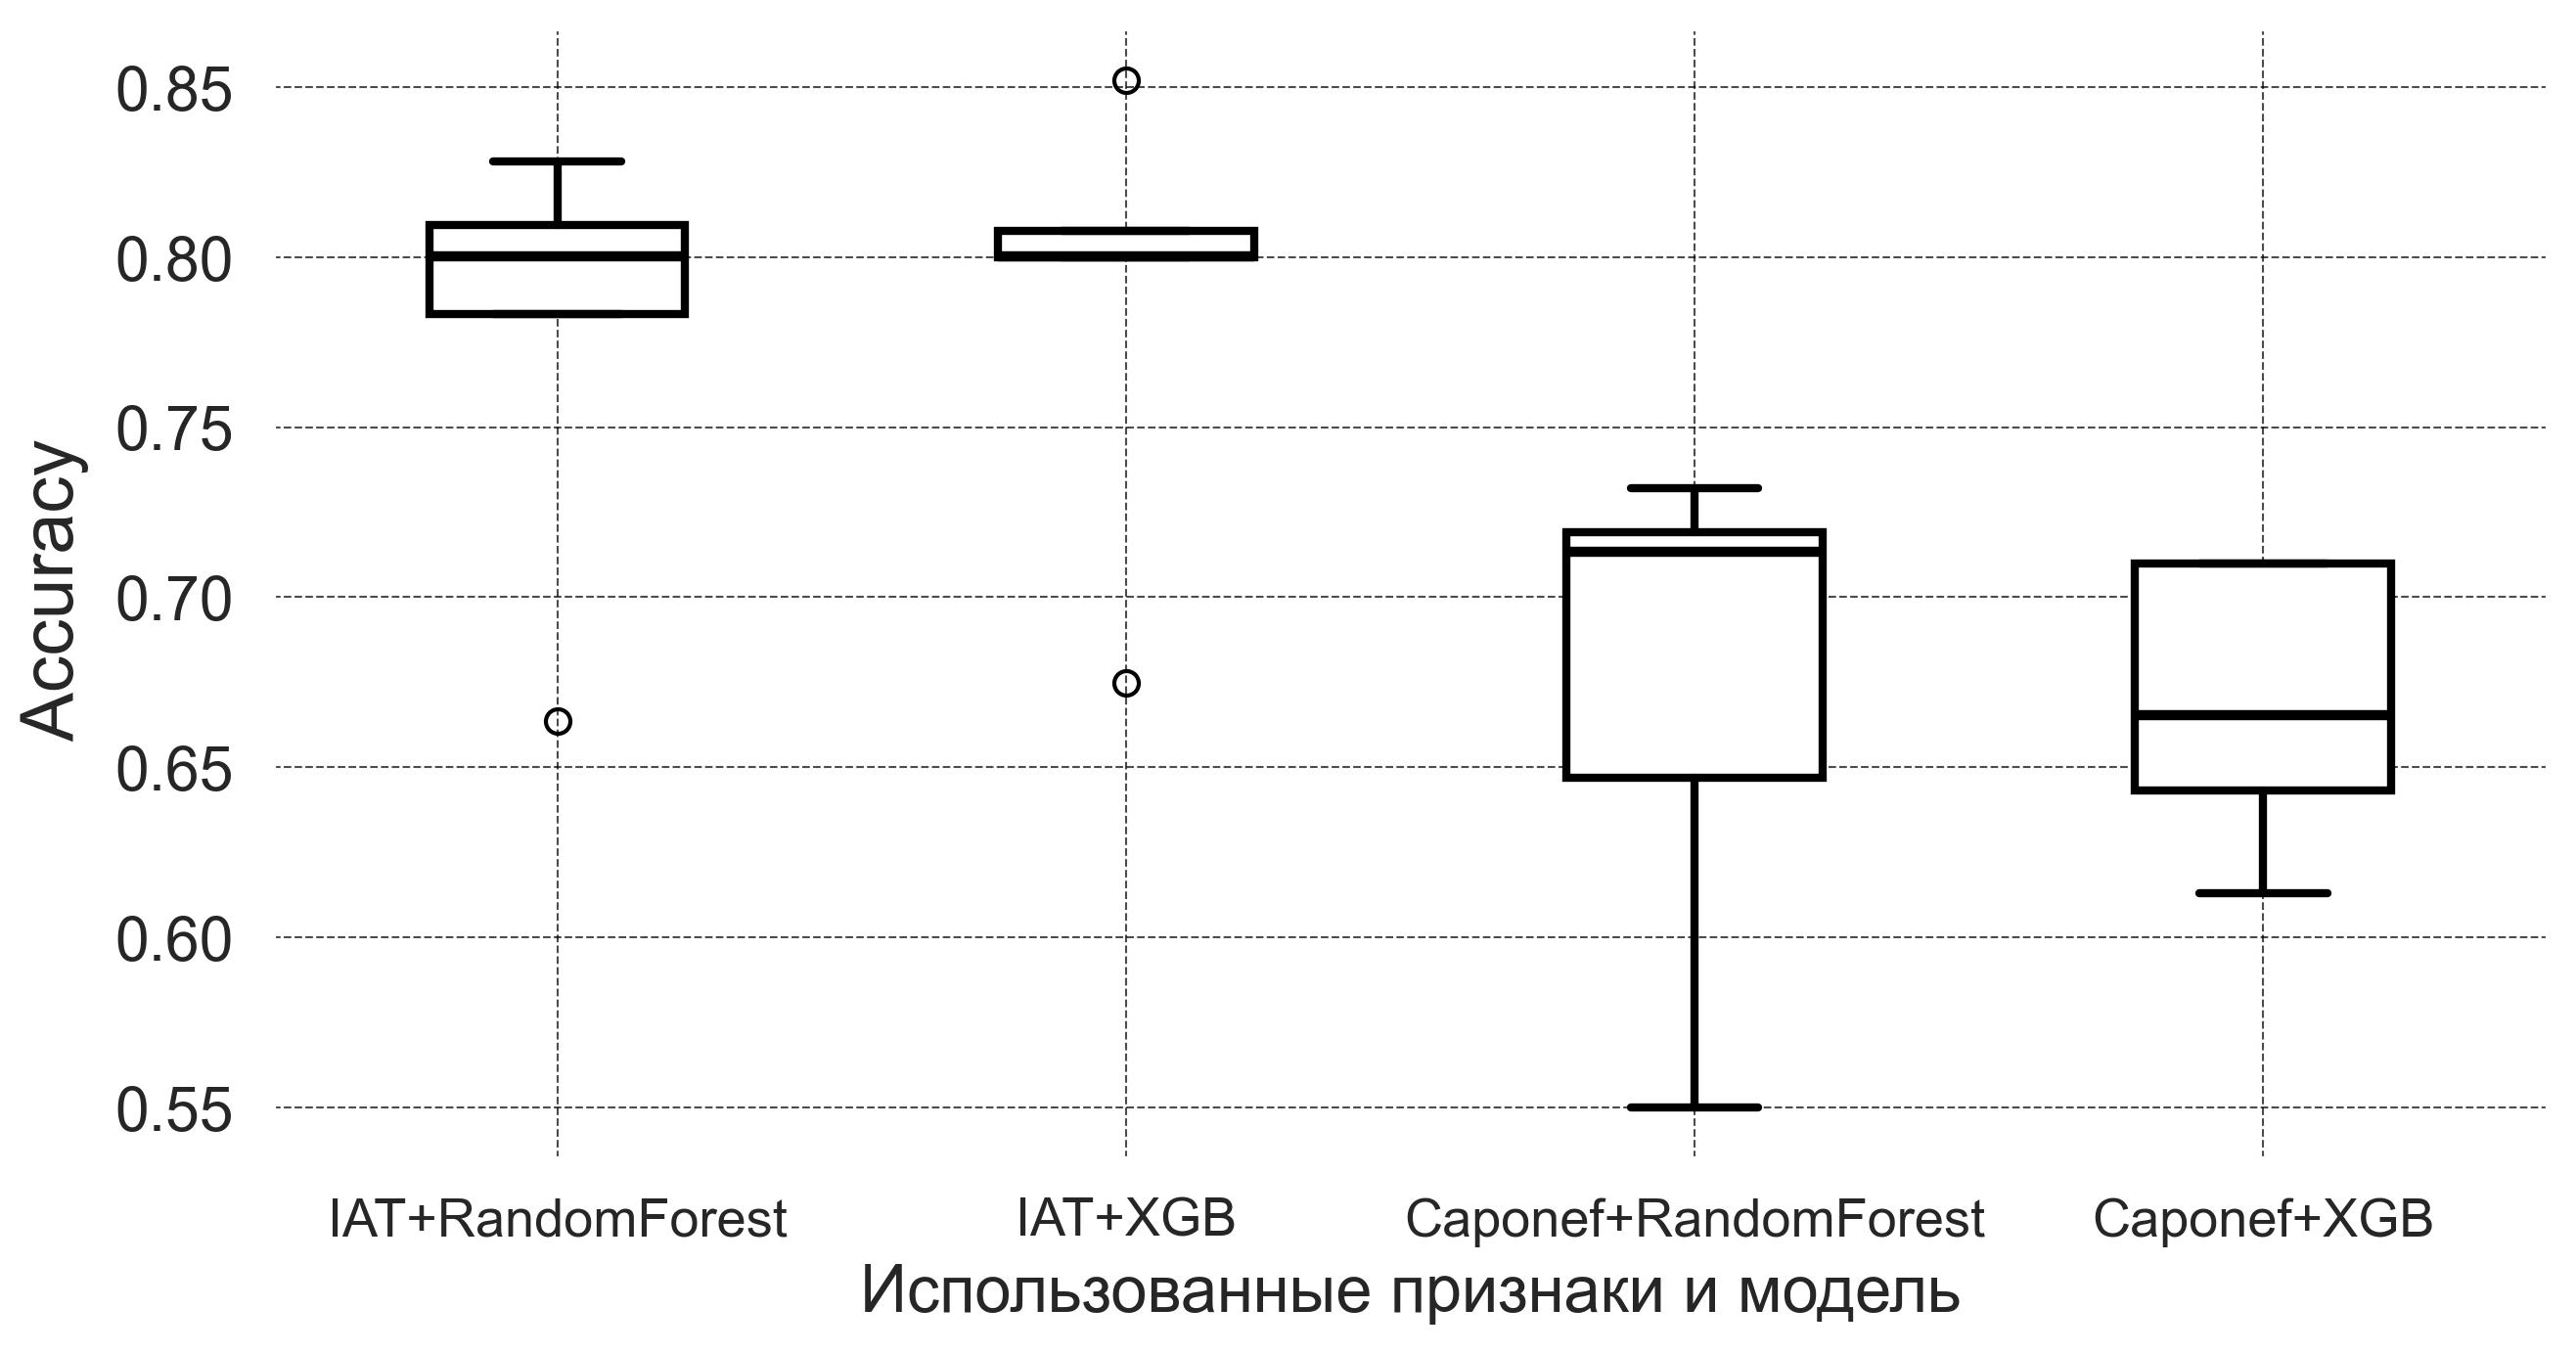
\includegraphics[width=0.7\linewidth]{images/caponef/iat_vs_cap_var_ru_bw}
	\caption{Результаты применения генерации признаков для алгоритмов случайного леса(RandomForest) и градиентного бустинга(XGB)}
	\label{fig:capo}
\end{figure}

В итоге, была проведена эмпирическая оценка двух методов генерации и преобразования признаков — AGMV и CAPoNeF — в условиях, отличных от оригинальных: методы были адаптированы по параметрам и протестированы на разнообразных наборах данных и архитектурах моделей машинного обучения. Эксперименты показали, что AGMV обеспечивает статистически значимое улучшение качества моделей, подтверждая свою универсальность и адаптивность, тогда как CAPoNeF систематически ухудшает результаты, что указывает на его чувствительность к параметрам или ограниченную применимость в задачах анализа трафика. Полученные результаты расширяют понимание границ применимости обоих методов и могут служить основой для обоснованного выбора стратегий генерации признаков в практических задачах и системах автоматизированного машинного обучения.


\underline{\textbf{Третья глава}} посвящена теме анализа сетевой инфраструктуры и производительности сетей. В ней описывается существующие системы по сбору данных о работе интернет сетей, а также рассматриваются вопросы постобработки  и калибровки получаемых данных. 


\underline{\textbf{В разделе 3.1}} описываются две наиболее крупные системы мониторинга интернет сетей: RIPE Atlas и  SamKnows. Рассмотрены их достоинства и недостатки, а также ключевые особенности доступности и распространенности по миру.

\begin{comment}

SamKnows — это платформа для мониторинга производительности интернет-сетей, предоставляющая пользователям и провайдерам возможность измерять качество соединения. Основанная в 2008 году компанией Cisco, система включила в себя решения на основе специализированного оборудования Whitebox (рисунок \ref{fig:sam}) и программного обеспечения, превращающего маршрутизаторы в измерительные зонды. Исследования подтверждают высокую точность данных SamKnows %\cite{Bagnulo2014Building}
, включая замеры скорости загрузки, задержек и потерь пакетов в реальных условиях. %\cite{Bajpai2015}, \cite{Sundaresan2012}.
 Однако платформа коммерческая — часть функций доступна только по подписке, что ограничивает её использование в науке. Также остаются вопросы конфиденциальности, так как собирается информация о сетевом трафике пользователей.


Еще одной популярной системой является RIPE Atlas %\cite{ripe}
, насчитывающая более 13 тысяч измерительных зондов по всему миру, более 700 <<Якорей>> (более мощные устройства серверного типа), а также свыше 76 тысяч активных пользователей (на момент января 2025). Среди партнеров системы присутствуют такие крупные компании как  Comcast и Console Connect. За 13 лет существования система значительно развилась: выпущено несколько версий аппаратных и программных зондов. На данный момент используется пятая версия зонда (рисунок \ref{fig:ripev5}) на базе устройств Turris Mox. %\cite{turris}.

\begin{figure}[htbp]
	\centering
	\begin{minipage}{0.49\textwidth}
		\centering
		
\includegraphics[width=\linewidth]{whitebox}
		\caption{Измерительное оборудование SamKnows - <<WhiteBox>>}
		\label{fig:sam}
	\end{minipage}
	\hfill
	\begin{minipage}{0.49\textwidth}
		\centering
		
\includegraphics[width=0.77\linewidth]{probev5}
		\caption{Аппаратный зонд RIPE Atlas - Probe V5}
		\label{fig:ripev5}
	\end{minipage}
\end{figure}

\end{comment}

RIPE Atlas была выбрана для дальнейших исследований благодаря возможности получения неагрегированных данных, в отличие от SamKnows, где доступны только усредненные метрики. %\cite{samknows}. 
Кроме того, RIPE Atlas децентрализована и предоставляет гибкость в проведении измерений, что делает её более подходящей для научного анализа. Также стоит подчеркнуть, что данная система, являясь некоммерческим проектом, созданным международным сообществом энтузиастов, представляет собой ценный инструмент для исследователей благодаря открытому и свободному доступу к результатам измерений.

Ключевым преимуществом таких систем является сбор данных из реальной сетевой инфраструктуры, а не смоделированного или лабораторного трафика. Примерами таковых могут служить многочленные наборы данных Канадского института кибербезопасности. %\cite{ddos}.


\underline{\textbf{Раздел 3.2}} более подробно описывает нюансы работы и особенности выбранной для исследований системы измерений - RIPE Atlas. В ходе работы с платформой RIPE Atlas было выявлено, что одним из факторов, ограничивающих исследования в области сетевого анализа, являются искажения, вносимые разными типами и версиями зондов. Например, первые две версии устройств добавляют значительные задержки. 

%Ещё одним фактором являются сетевые условия: RIPE Atlas не проверяет доступную пропускную способность перед измерениями, однако можно учитывать время суток для построения гипотез об искажениях. Также важно учитывать суточную активность некоторых устройств — например, они могут включаться и выключаться в определённое время.

\begin{comment}

Система RIPE Atlas использует балльную модель: пользователи накапливают баллы, устанавливая зонды, и тратят их на запуск измерений. Также доступ и баллы начисляют спонсорам и партнерам RIPE.
\end{comment}
 Система поддерживает следующие типы измерений: PING (время отклика), TRACEROUTE (время соединения между промежуточными адресами), DNS (производительности DNS-серверов), TLS (скорости работы сертификатов безопасности), HTTP (скорость обработки простых http-запросов)и NTP (отслеживание процесса синхронизации часов). <<Стоимость>> измерений зависит от типа и параметров (например, таких как частота и длительность). Данные предоставляются в формате JSON через API или веб-интерфейс.

\begin{comment}

\begin{table}[htbp]
	\caption{Стоимость в баллах системы RIPE Atlas различных видов сетевых измерений в расчете за один запрос к одному устройству}
	\begin{center}
		\begin{tabular}{|c|c|}
			\hline
			\textbf{Тип измерения} & \textbf{Стоимость} \\
			\hline
			TRACEROUTE & 60 \\
			\hline
			DNS (UDP) & 20 \\
			\hline
			DNS (TCP) & 40 \\
			\hline
			TLS & 20 \\
			\hline
			PING (ipv4/ipv6) & 6 \\
			\hline
			NTP & 20 \\
			\hline
			HTTP & 20 \\
			\hline
		\end{tabular}
		\label{prices}
	\end{center}
\end{table}
\end{comment}

Анализ данных показал, что устройства разных версий вносят различную дополнительную задержку. Например, при измерении TRACEROUTE до сервера gov.ru были задействованы 480 зондов с 8 версиями прошивок и ПО. Наибольшие задержки демонстрируют старые аппаратные версии V1 и V2. Современные версии V3, V4, Anchor и программные зонды показывают задержки менее 1 мс. Результаты представлены на рисунке \ref{probe_offset}.

\begin{figure}[h]
	\centering
	
\includegraphics[width=0.9\linewidth]{probe_offset.png}
	\caption{Картина распределений времени отклика первого узла маршрута для различных типов и поколений устройств RIPE Atlas}
	\label{probe_offset}
\end{figure}

Устройства V1 и V2 существенно отличаются по характеристикам от V3 и V4. В связи с этим необходимо учитывать влияние аппаратной реализации при анализе данных. В новых выборках доля старых версий прошивок невелика (<5\%), поэтому основное внимание уделялось аномалиям, вызванных различиями между аппаратными версиями.

\underline{\textbf{В разделе 3.3}} представлены результаты калибровки данных путем оценки систематической ошибки. 

Для устранения влияния оборудования в измерениях RTT было решено провести калибровку. Применение калибровки путем оценки систематической ошибки позволило повысить точность показателей, однако статистические различия между распределениями остались значимыми (вероятность получить такие же или ещё большие отклонения при условии нулевой гипотезы (здесь и далее для краткости p-value) $p-value < 0,01$). 
Результаты калибровки приведены в таблице \ref{calib1}.


%Программные зонды показали высокую дисперсию во времени отклика и требуют более сложной калибровки, что делает их использование на текущем этапе нецелесообразным.


\begin{table*}[!ht]
	\centering
	\caption{Результаты калибровки, выраженные в показаниях статистических тестов Манна–Уитни (U-test) и Колмогорова–Смирнова (KS-test). U/D - значение статистики в тестах}
	\begin{tabular}{|c|c|c|c|c|c|c|c|}
		\hline
		Стат. & \multirow{3}{*}{Этап} & \multicolumn{6}{c|}{Тип калибруемого устройства} \\ \cline{3-8}
		Тест & & \multicolumn{2}{c|}{System V1} 
		& \multicolumn{2}{c|}{System V2} 
		& \multicolumn{2}{c|}{System V4} \\ \cline{3-8}
		& & U/D & p-value
		& U/D & p-value
		& U/D  & p-value \\ \hline
		KS-test & До              & 1,0        & 0,0        & 1,0         & 0,0         & 0,89        & 0,0        \\ \hline
		KS-test & \textbf{После}  & 0,249      & 2,6e-42    & 0,23        & 5,7e-124    & 0,058       & 4,5e-19    \\ \hline
		U-test  & До              & 13e6       & 0,0        & 53e6        & 0,0         & 168e6       & 0,0        \\ \hline
		U-test  & \textbf{После}  & 6e6        & 0,0003     & 24e6        & 1,8e-14     & 85e6        & 0,0008     \\ \hline
	\end{tabular}
	\label{calib1}
\end{table*}

На основе тестов и визуального анализа сделан вывод о значительном отличии форм распределений у программных зондов и <<Якорей>>. Было предложено разработать метод калибровки на основе преобразования распределений (Distribution Transforming).


\underline{\textbf{Раздел 3.4}} описывает анализ одного из метода преобразования распределений - Квантиль Трансформер (Quantile Transformer).


Квантильтрансформер позволяет переводить данные в равномерное или нормальное распределение и хорошо работает с ненормально распределенными данными. % \cite{MingXuan_2023_01, Varoquaux_2015_06}.
Для оценки эффективности метода проводились эксперименты с использованием синтетических данных из гамма-распределения (\ref{gamma}) и линейных деформаций. Оптимальные параметры — 24 и 43 квантиля для эталонной и калибруемой выборок соответственно — были применены к наблюдаемым данным. Визуальный и метрический анализ  подтвердил улучшение соответствия эталонному устройству (устройства System: V3). %(рисунок \ref{fig:qt2})

\begin{equation}
	f(x) =  x^{k-1} \frac{e^{-x/\theta}}{\theta^k \Gamma(k)}
	\label{gamma}
\end{equation}

\begin{comment}
	\begin{figure}[ht]
		\centerfloat{
			\hfill
			\subcaptionbox{}{%
				
\includegraphics[width=0.49\linewidth]{qtransf/test_before}}
			\hfill
			\subcaptionbox{}{%
				
\includegraphics[width=0.49\linewidth]{qtransf/test}}
			\hfill
		}
		\caption{Пример применения квантильтрансформера на данных RIPE Atlas. а) - Исходный вид выборки эталонного и калибруемого устройства, б) - Выборка после калибровки с параметрами, подобранными на синтетических данных}
		\label{fig:qt2}
	\end{figure}
\end{comment}

Несмотря на положительные результаты, метод требует значительных вычислительных затрат и тонкой настройки числа квантилей. С ростом разнообразия устройств его применимость усложняется, поэтому дальнейшее исследования квантильтрансформера не проводилось.

\underline{\textbf{Раздел 3.5}} посвящен анализу параметрических распределений и их применимости для калибровки полученных данных.

Визуальный анализ данных показал различия в формах распределений между типами устройств, несмотря на отсутствие статистически значимых отличий по критерию Манна–Уитни. 

Это обосновывает необходимость более точной калибровки, основанной не только на средних значениях, а на анализе всего распределения. Для этого использовался подход с параметрическими распределениями.

Были проверены гипотезы о нормальности и логнормальности с помощью тестов Шапиро–Уилка и $\chi^2$, но они не позволили принять гипотезу о принадлежности данных к генеральной совокупности(ГС) этих распределений. Поэтому для оценки распределений применили ядерную оценку плотности (KDE) с гауссовым ядром и правилом Скотта. %(рисунок \ref{fig:kde}).

\begin{comment}
	\begin{figure}[h]
		\centering
		
\includegraphics[width=0.7\linewidth]{calib/kde}
		\caption{KDE-оценка плотности вероятности для времени отклика}
		\label{fig:kde}
	\end{figure}
\end{comment}


Далее оценили параметры для распространённых распределений: нормального, логнормального, смещённого нормального, обобщённого нормального и гамма-распределения. %Пример приближения показан на рисунок \ref{fig:examplekde}.

\begin{comment}

\begin{figure}[h]
	\centering
	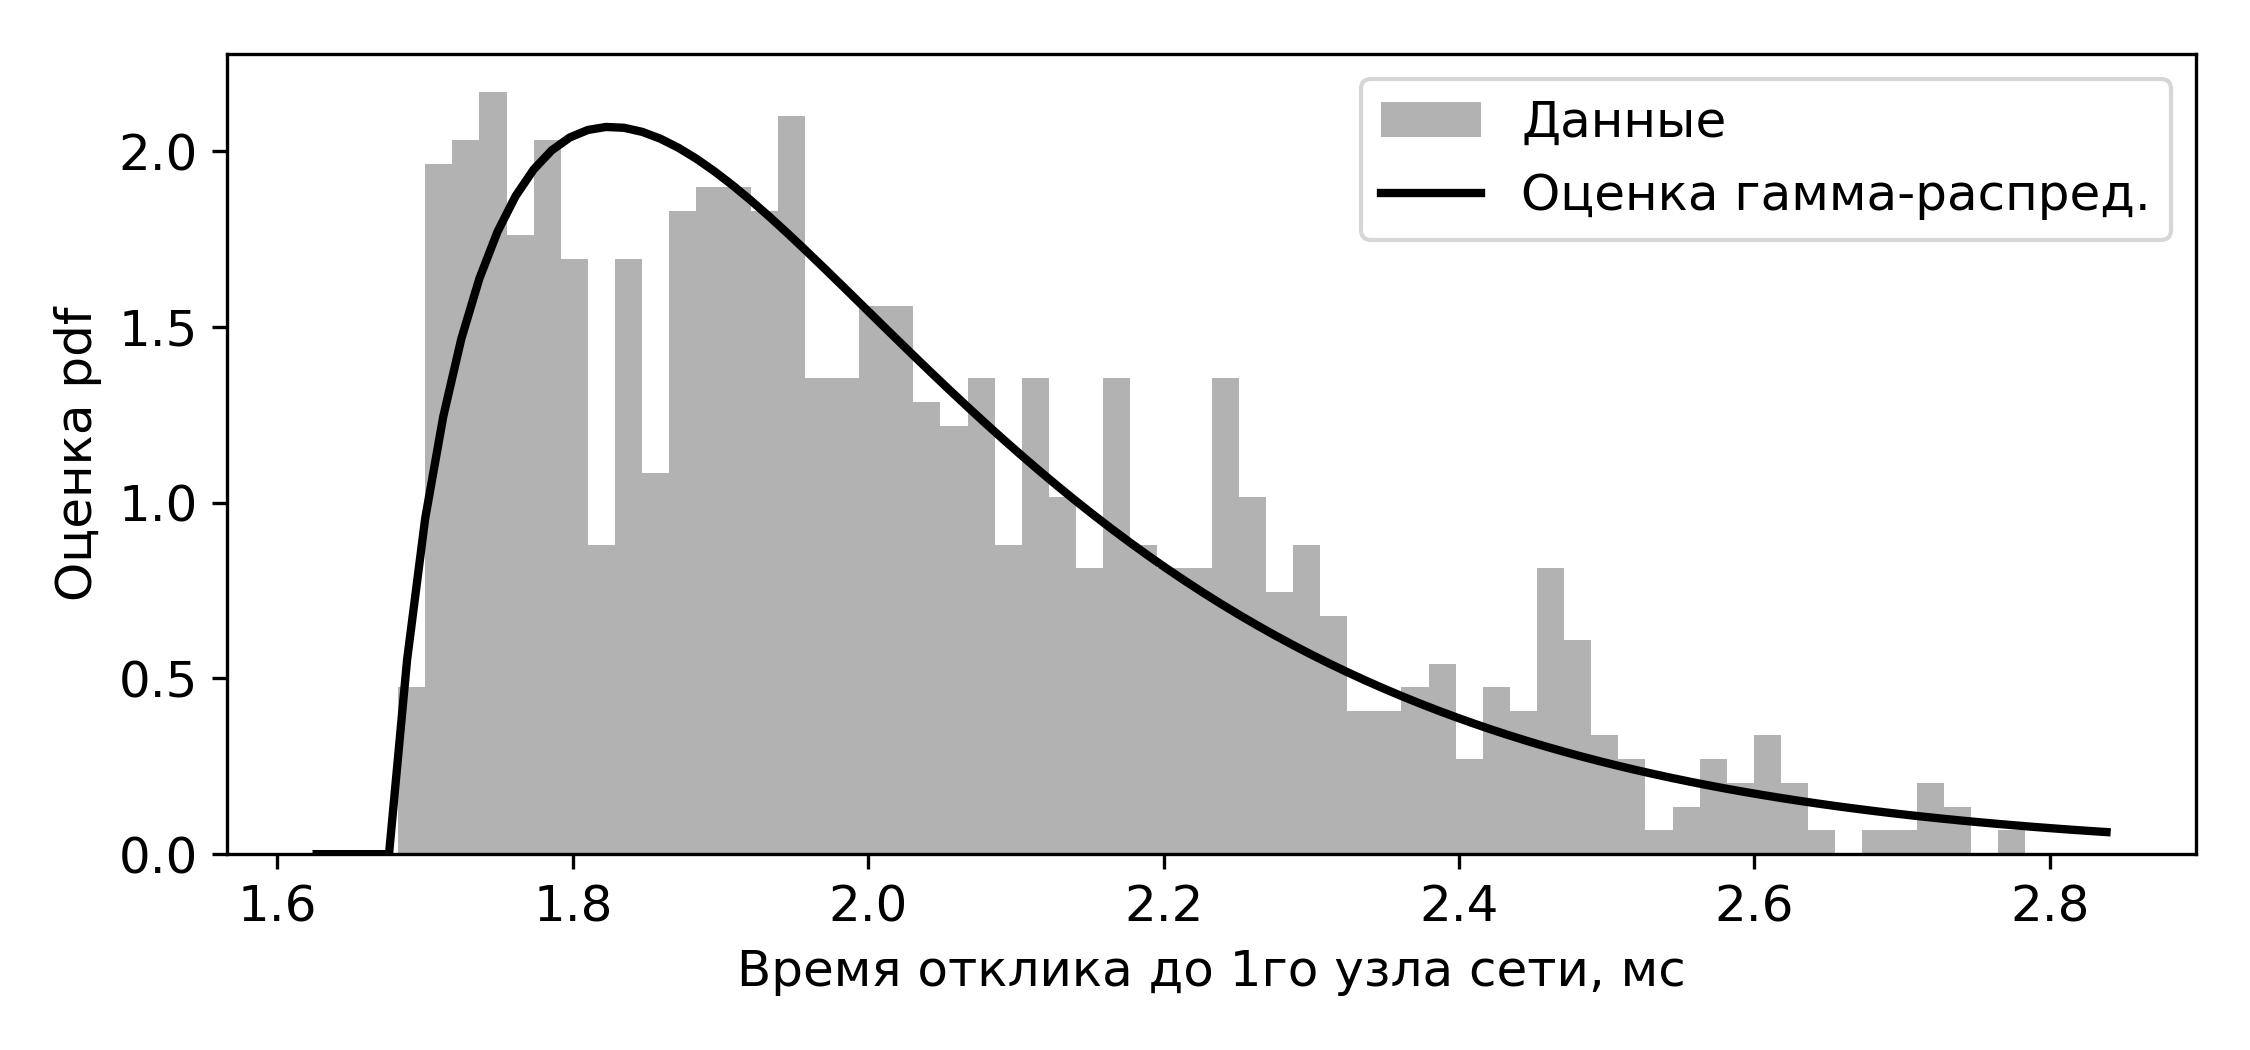
\includegraphics[width=0.7\linewidth]{images/calib/example_kde}
	\caption{Пример приближения pdf с использованием гамма-распределения}
	\label{fig:examplekde}
\end{figure}
\end{comment}

Сравнение моделей выполнено с помощью дивергенции Джефриса (\ref{jefrice}) — симметричной версии KL-дивергенции (\ref{kl_deiv}).

\begin{equation}
	D_{KL}(P||Q) =  \int_X p \cdot \log \frac{p}{q} d\mu
	\label{kl_deiv}
\end{equation}
\begin{equation}
	D_{J}(P||Q) =  \frac{1}{2} D_{KL}(P||Q) + \frac{1}{2} D_{KL}(Q||P)
	\label{jefrice}
\end{equation}

Результаты сравнения приведены в таблице \ref{pdf_compare} и на рисунке \ref{fig:kderesults}. Как можно отметить, лучшие приближения  были достигнуты с использованием логнормального и гамма-распределения. Поэтому в дальнейшем анализе использовались данные параметрические распределения.


\begin{table*}[!ht]
	\centering
	\caption{Результаты сравнения наблюдаемых данных и рассматриваемых параметрических распределений, выраженные в
		расстоянии (дивергенции) Джефриса от табличного распределения до оценки по KDE. Обозначения распределений: lognormal - логнормальное, skewnorm - смещенное нормальное, gennorm - обобщенное нормальное}
	\begin{tabular}{|c|c|c|c|>{\centering\arraybackslash}p{1.8cm}|c|}
		\hline
		 lognormal & skewnorm & gamma & gennorm     & Тип устройства & Лучшее \\ \hline
		 0,101 & 0,271 & 0,153 & 0,823 & system: V4 & lognormal \\ \hline
		 0,050 & 0,411 & 0,081 & 0,458 & system: V3 & lognormal \\ \hline
		 0,026 & 0,531 & 0,018 & 0,064 & Software   & gamma \\ \hline
		 0,056 & 0,402 & 0,032 & 0,091 & system: V1 & gamma \\ \hline
	   	0,066 & 0,167 & 0,022 & 0,603 & system: V2  & gamma \\ \hline
		 0,125 & 0,461 & 0,049 & 0,109 & Anchor     & gamma \\ \hline
	\end{tabular}
	\label{pdf_compare}
\end{table*}



\begin{figure}[h]
	\centering
	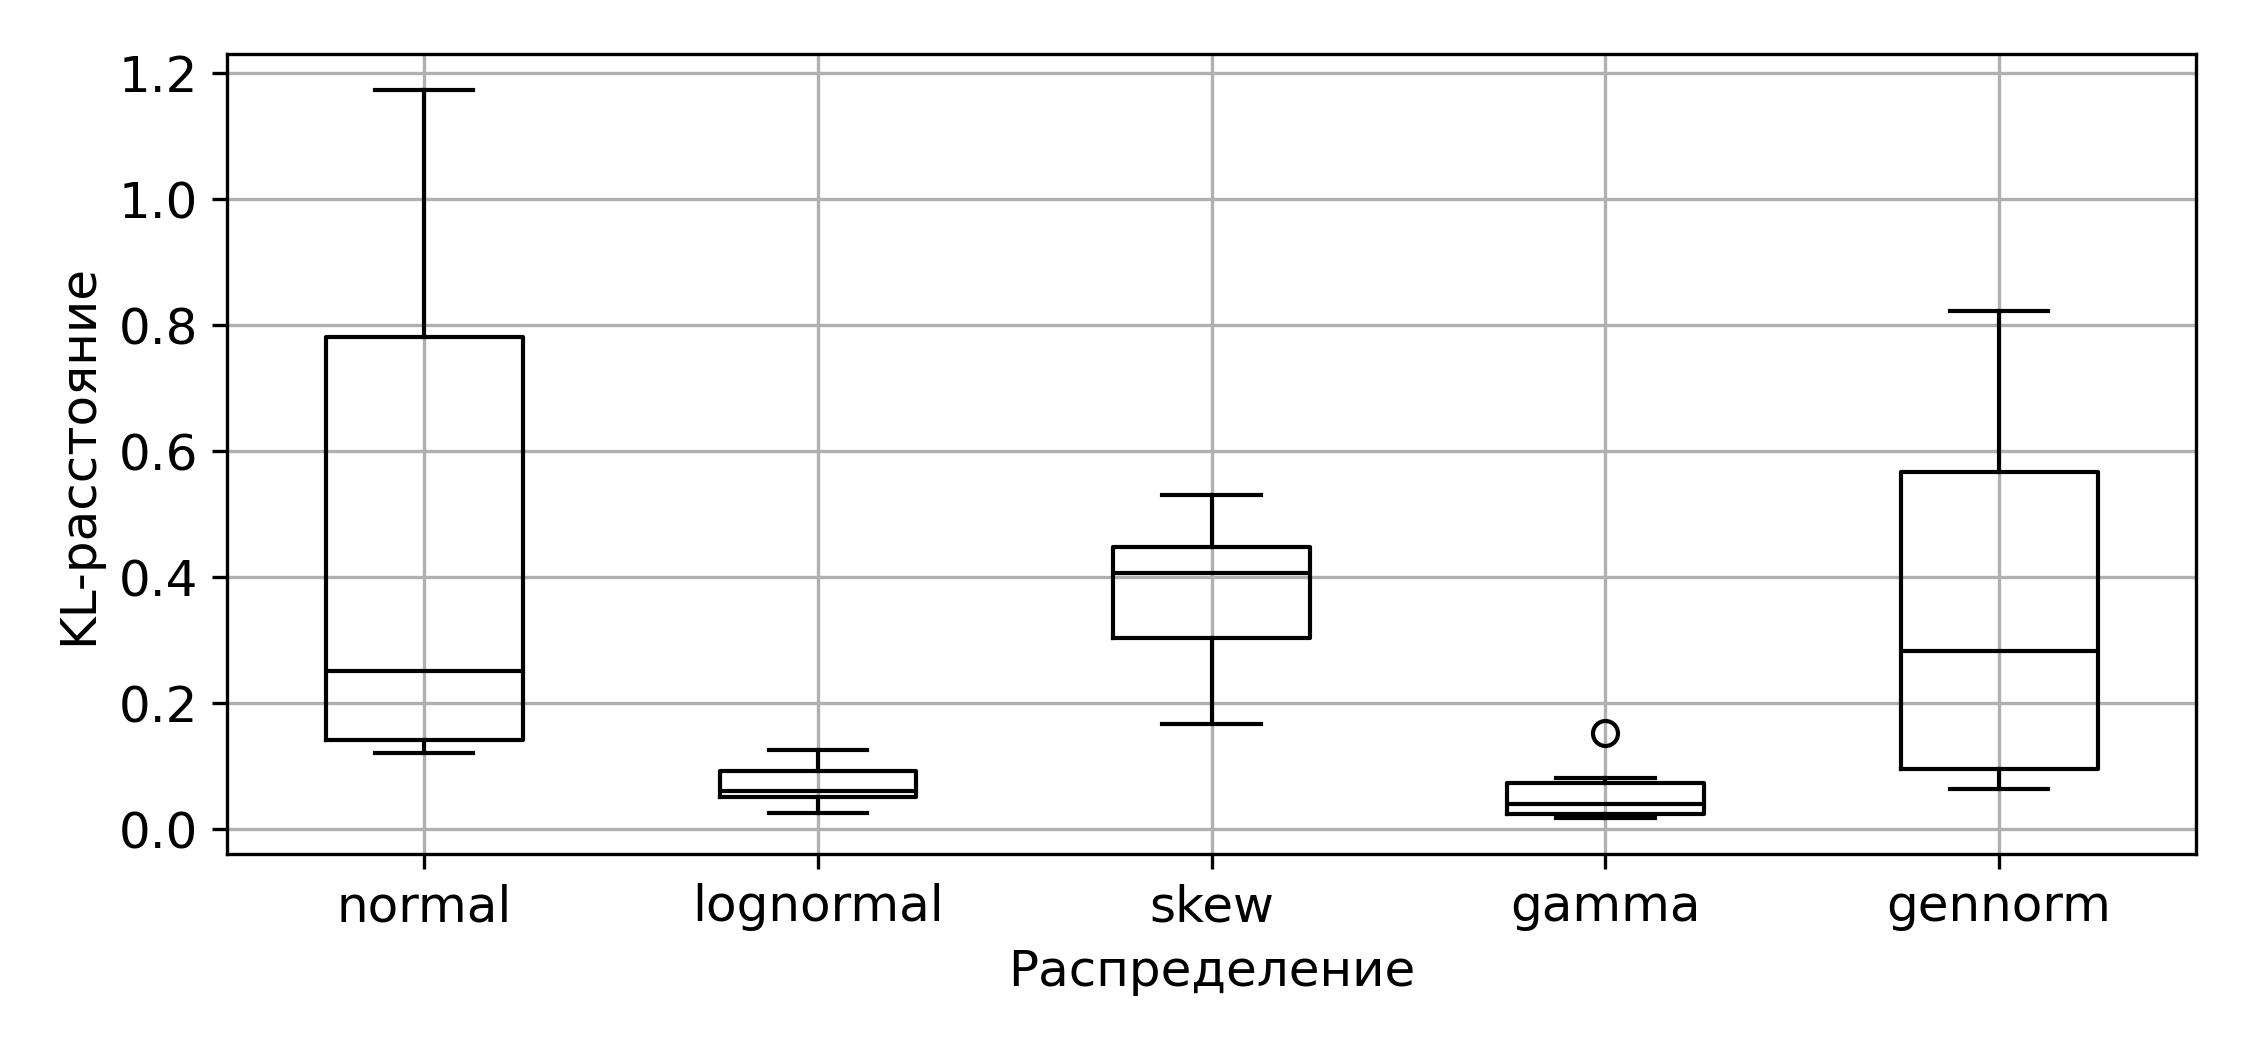
\includegraphics[width=0.7\linewidth]{images/calib/kde_results}
	\caption{Сравнение KDE и оценок параметрических распределений}
	\label{fig:kderesults}
\end{figure}

Для калибровки было использовано следующее преобразование распределений:

\begin{equation}
	x_{calib} = F_{ref}^{-1}(F_{obs}(x)) ,
	\label{сalib_table}
\end{equation}
где $F_{ref}$ — функция распределения эталонного устройства (system: V3), а $F_{obs}$ — калибруемого. Примеры результатов применения описанного метода для аппаратных устройств версии V3 и V4 приведены на рисунке \ref{fig:before_after_gamma}.


\begin{figure}[ht]
	\centerfloat{
		\hfill
		\subcaptionbox[List-of-Figures entry]{\label{fig:before_gamma}}{%
			
\includegraphics[width=0.49\linewidth]{calib/before_gamma}}
		\hfill
		\subcaptionbox{ \label{fig:after_gamma}}{%
			
\includegraphics[width=0.49\linewidth]{calib/after_gamma}}
		\hfill
	}
	\caption{Данные с устройств <<system:V4>> и <<system:V3>>: а) - до проведения калибровки, б) - после калибровки с использованием гамма-распределения}\label{fig:before_after_gamma}
\end{figure}



Сравнение методов выполнено по дивергенции Джефриса и расстоянию Вассерштейна (\ref{eq:wass}):

\begin{equation}
	W_1(P,Q) = \int_{-\infty}^{+\infty} |P(x)-Q(x)|dx ,
	\label{eq:wass}
\end{equation}
где $P(x)$ и $Q(x)$ - это функции распределения сравниваемых распределений.

Особенно сильный эффект наблюдается для устройств Anchor и Software, где распределения имеют значительные различия. Преобразование распределений показало кратно лучшие результаты по сравнению с простой оценкой систематической ошибки (shift) (рисунок \ref{fig:kl2}, \ref{fig:was2}).

\begin{figure}[!ht]
	\centering
	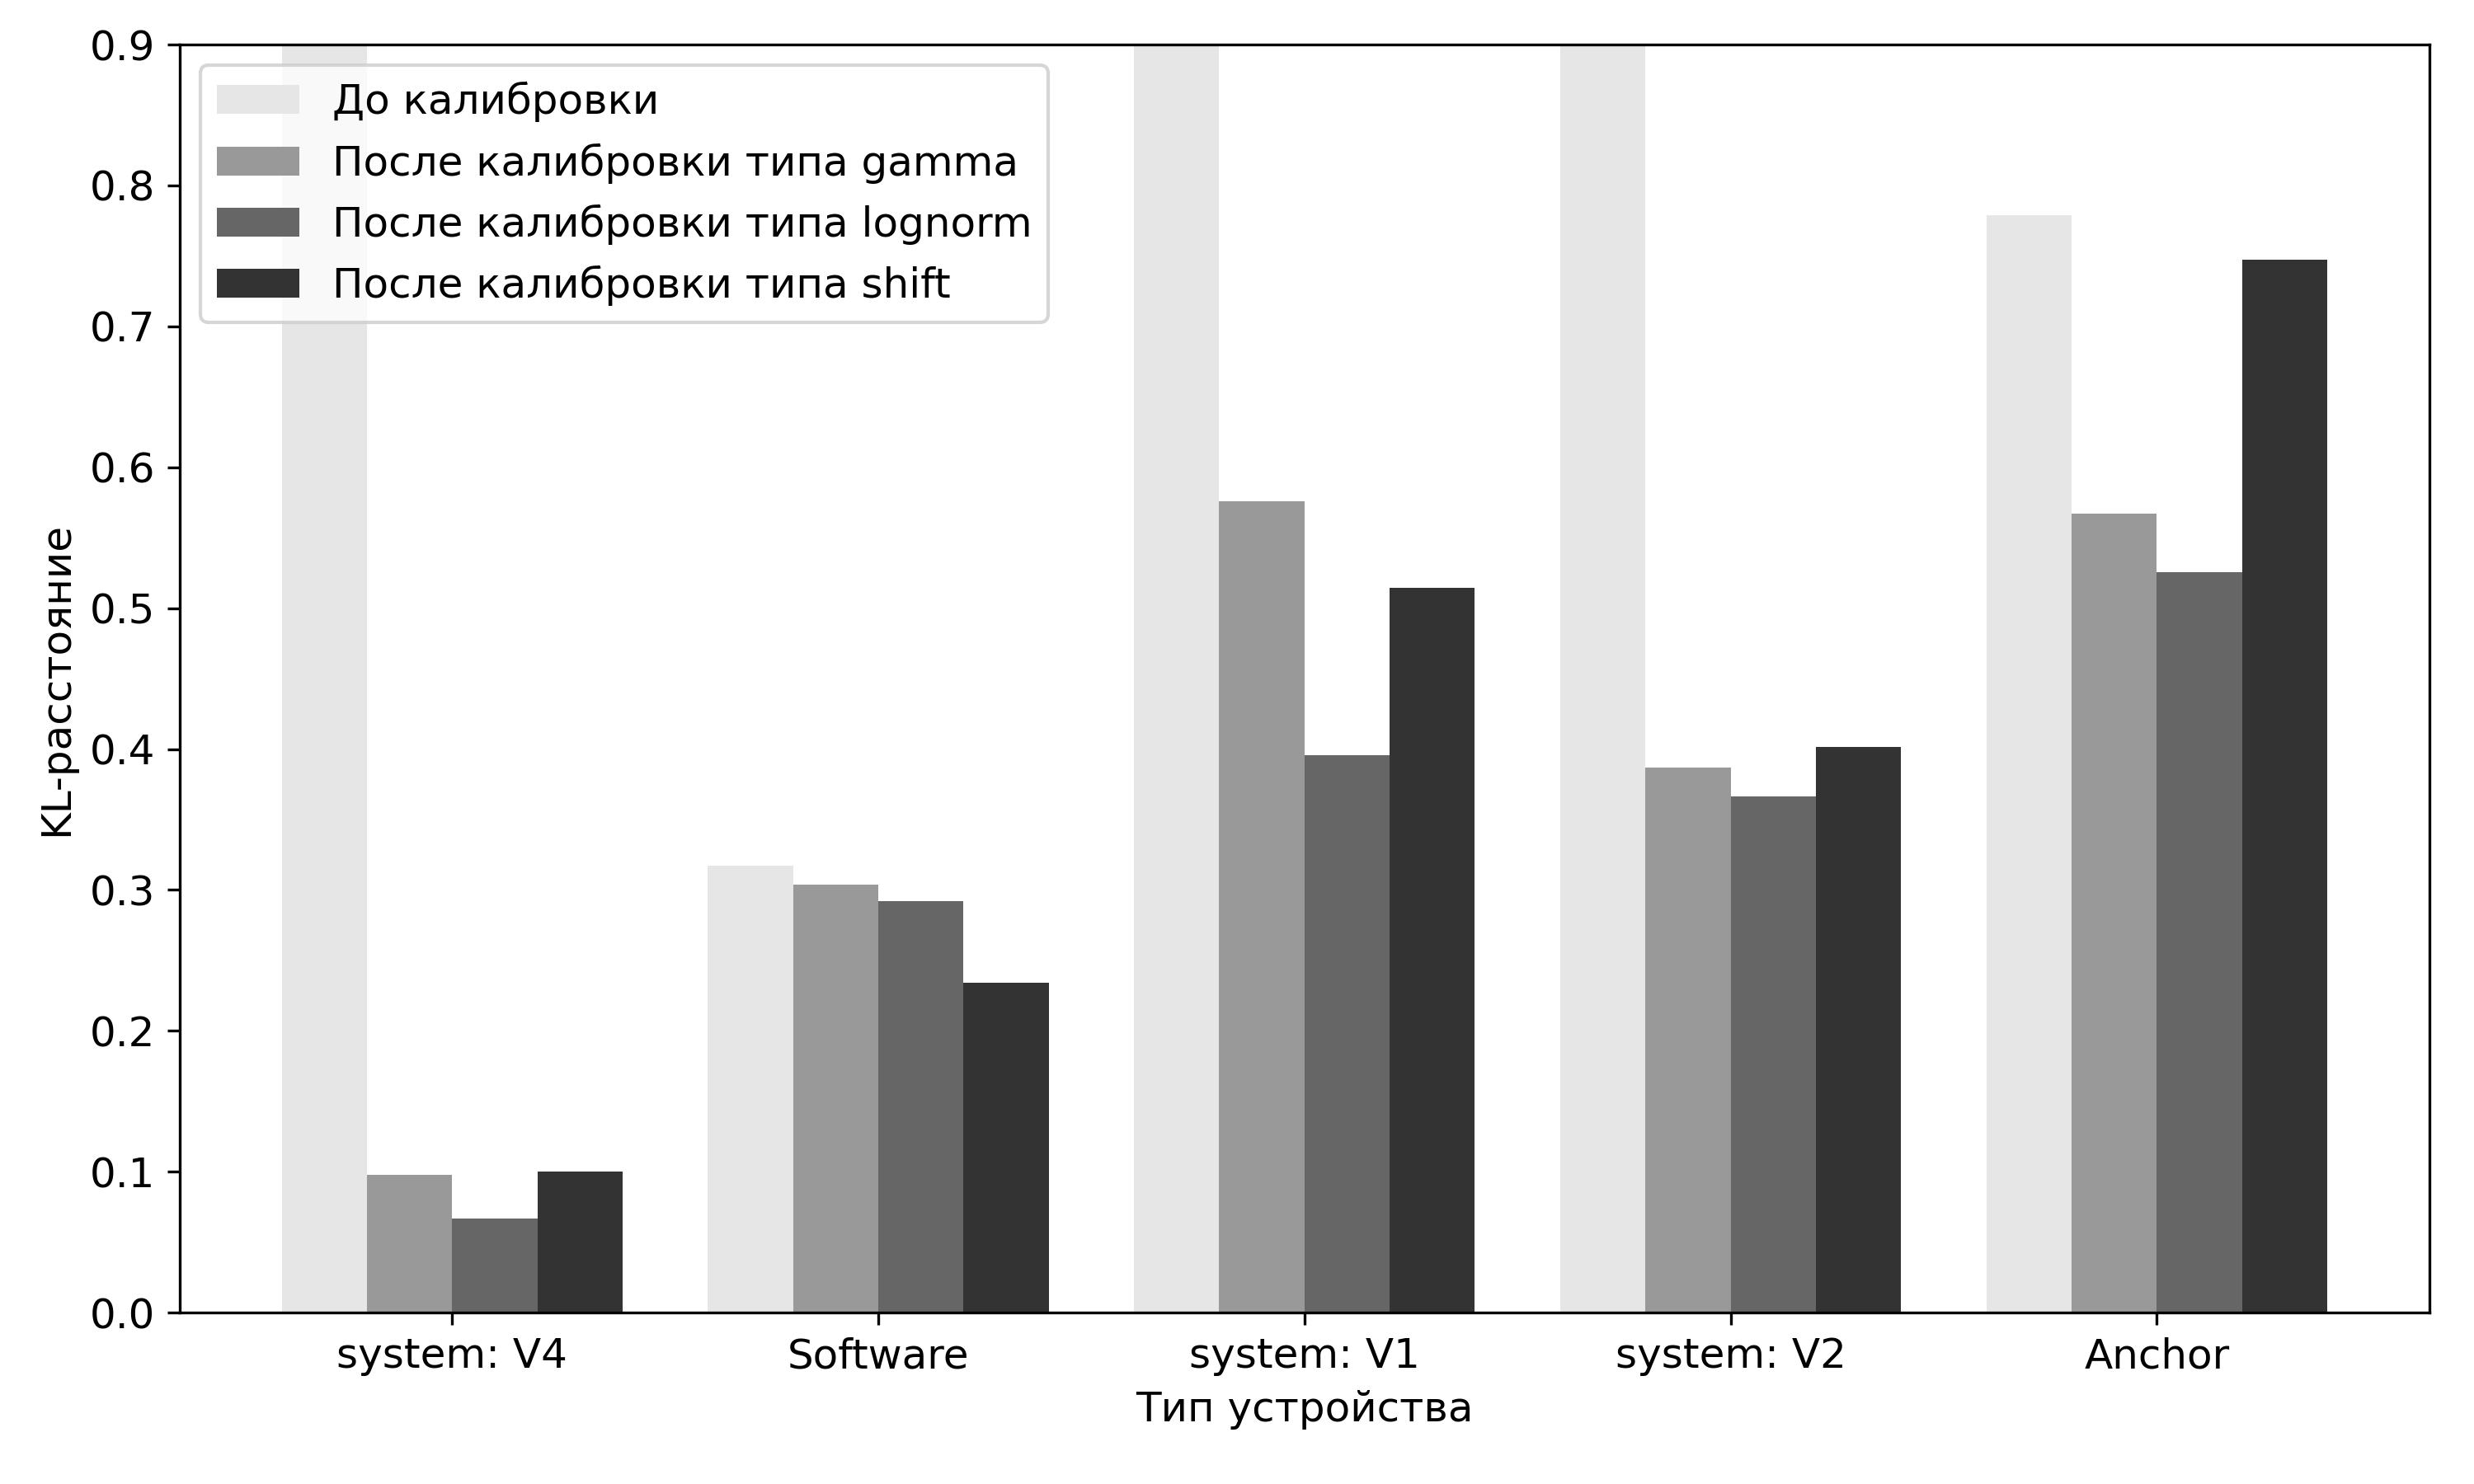
\includegraphics[width=0.7\linewidth]{../images/calib/KL_2}
	\caption{Сравнение дивергенции Джефриса до и после применения калибровки (увеличенный масштаб).}
	\label{fig:kl2}
\end{figure}

\begin{figure}[!ht]
	\centering
	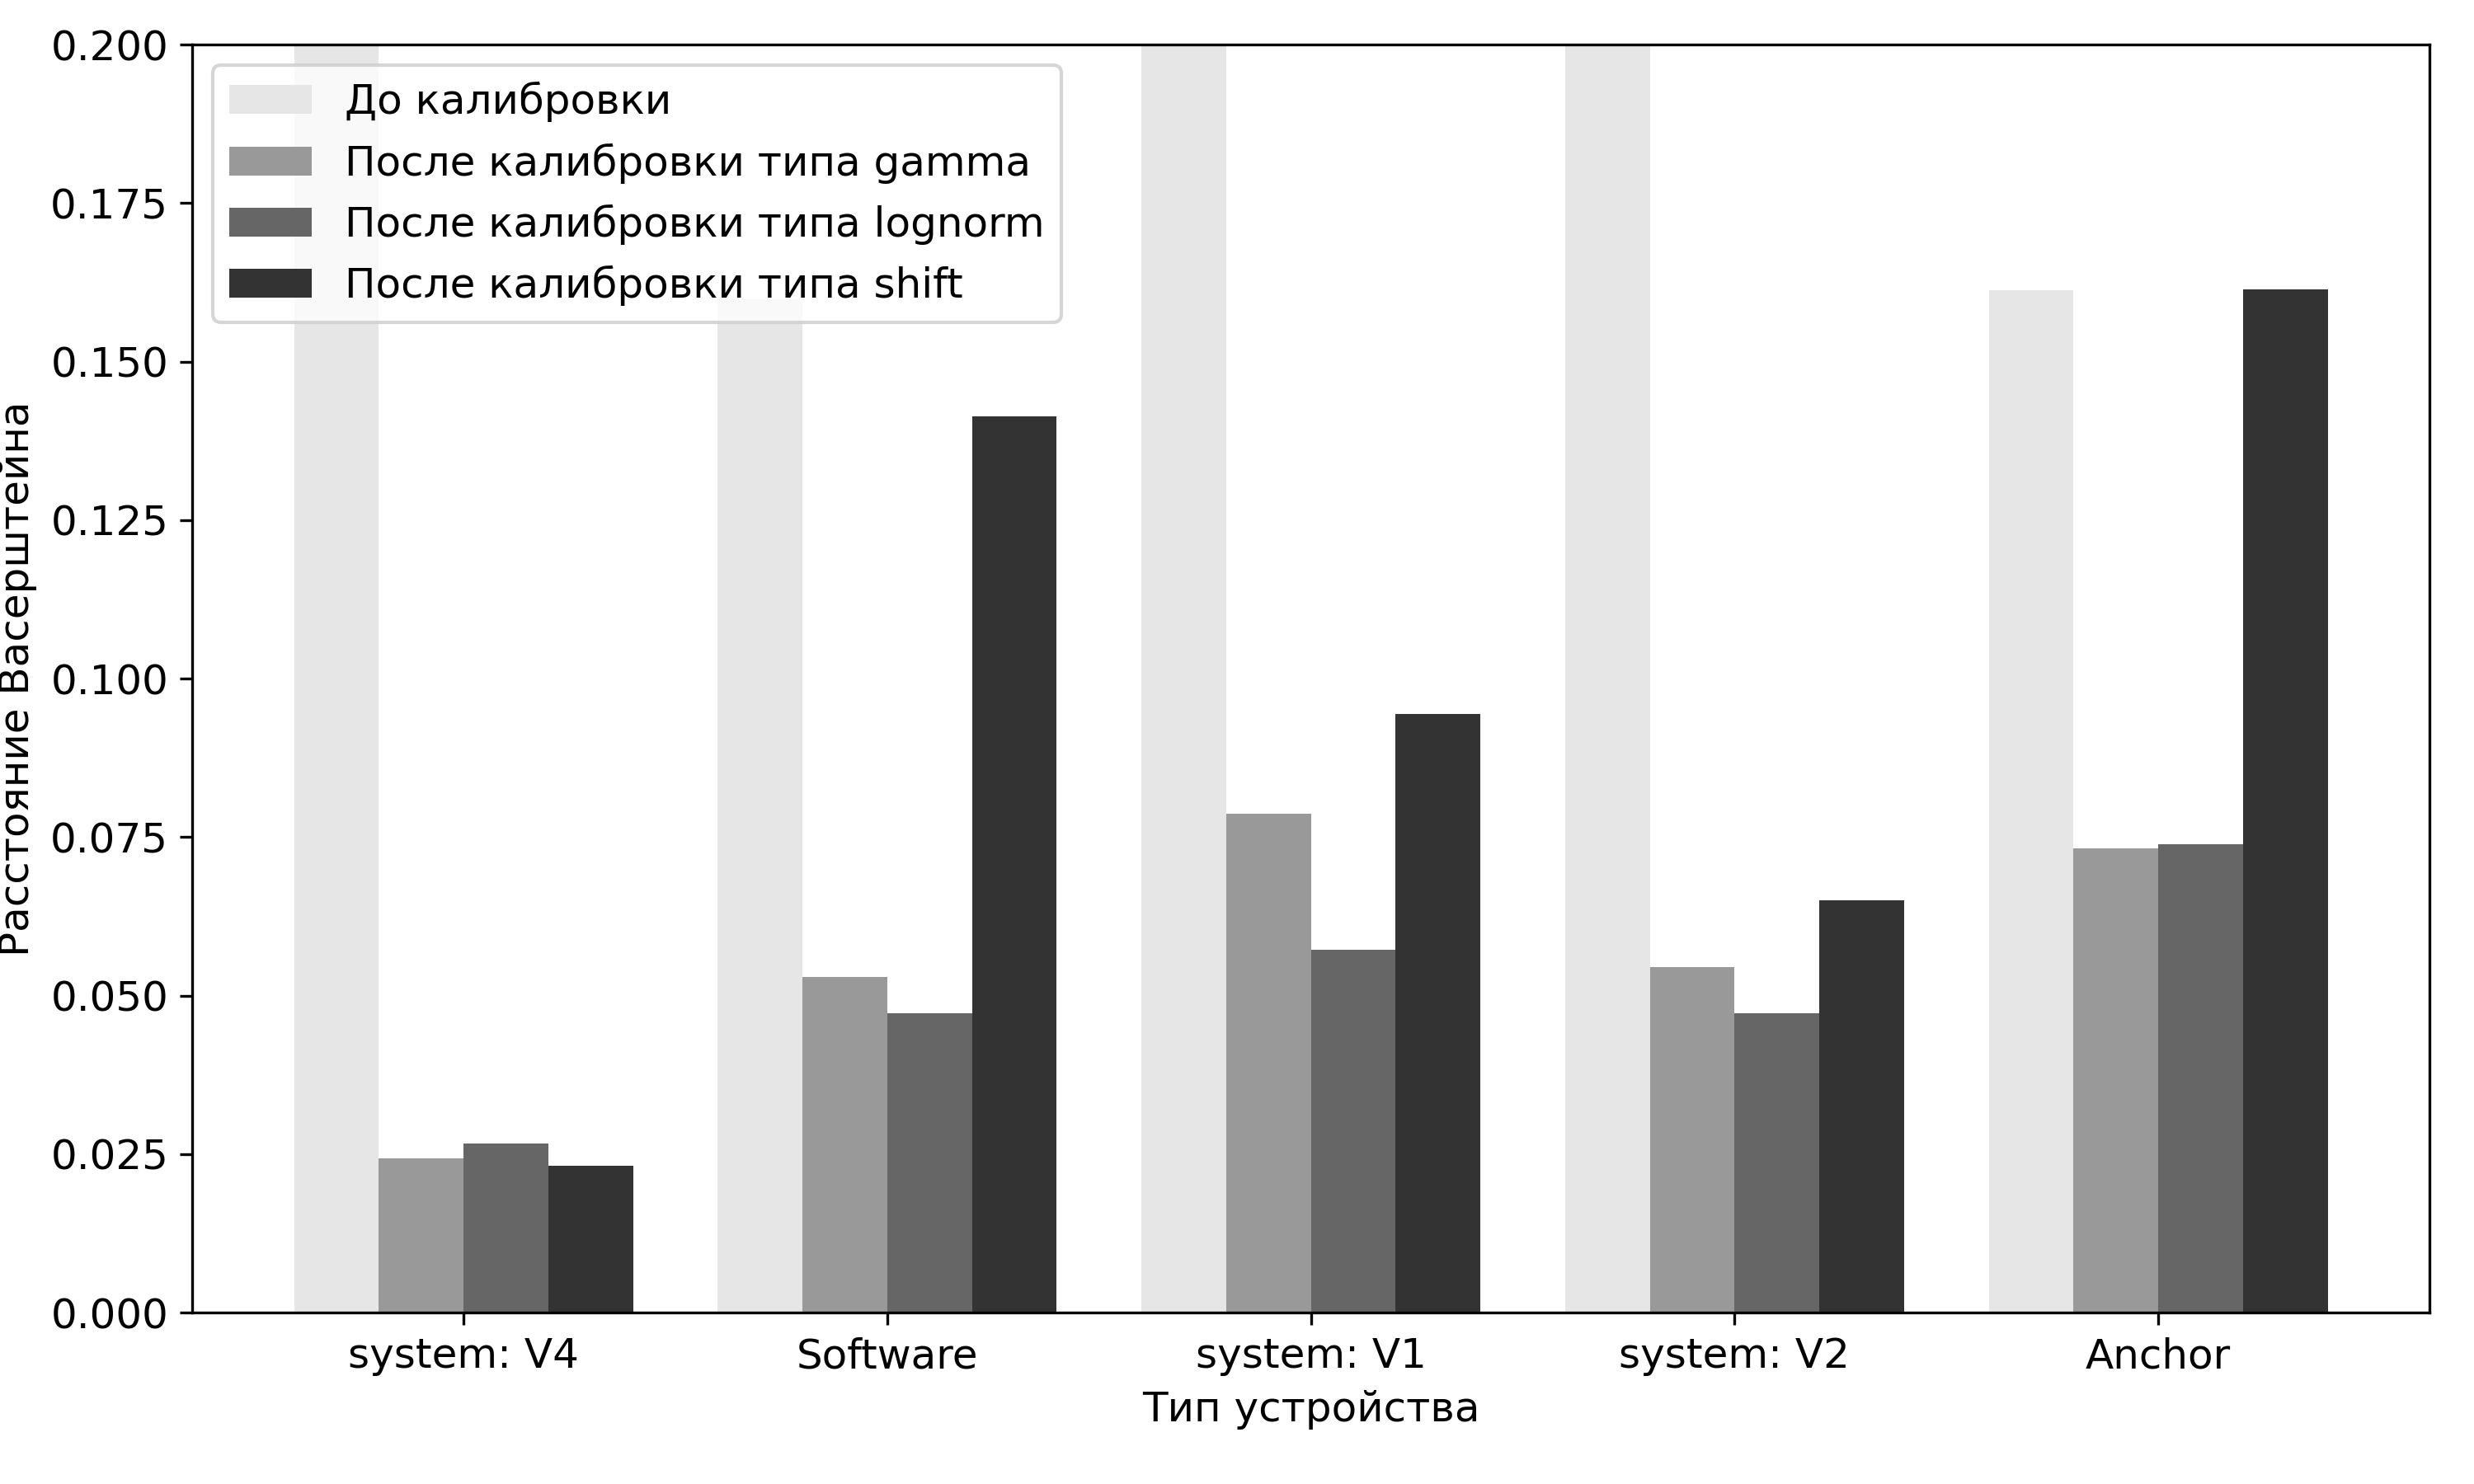
\includegraphics[width=0.7\linewidth]{../images/calib/was_2}
	\caption{Сравнение Расстояния Вассерштейна до и после применения калибровки (увеличенный масштаб).}
	\label{fig:was2}
\end{figure}

В итоге, предложен новый метод калибровки, основанный на аппроксимации и трансформации распределений, который превосходит простую оценку сдвига, особенно при значительных отличиях формы распределений. Тем не менее, для данного подхода видятся векторы его развития и улучшения: исследование других географических зон, анализ эффективности на новом типе устройств после роста его количества до сравнимого с предыдущими поколениями, а также исследование сходимости и оптимизации. % Также стоит подчеркнуть его меньшую вычислительную стоимость в сравнении с Квантиль Трансформером.


\underline{\textbf{Четвертая глава}} содержит в себе результаты анализа данных о времени отклика, полученных в ходе измерений, проведенных с помощью системы RIPE Atlas, а также результаты применения методов оценки состояния узлов и загруженности сети. 


\underline{\textbf{Раздел 4.1}} описывает характер проводимых измерений: период, частота и тип проводимых измерений сети интернет.

Для анализа доступности портала госуслуг gosuslugi.ru на территории РФ в период с 2024-05-26 по 2024-06-11 (16 суток) проводились измерения времени отклика c использованием 506 зондов RIPE Atlas. Сбор данных проводился с периодом в 20 минут (1200 секунд) путем отправки 4 пакетов и фиксированием среднего времени до пришедшего отклика. Всего было получено более 550 тысяч результатов измерений. Наибольшее количество устройств находилось в Центральном федеральном округе (246 шт.). %(рисунок \ref{fig:map}).

\begin{comment}
	\begin{figure}[h]
		\centerline{
\includegraphics[width=0.8\linewidth]{time_series/map}}
		\caption{Места размещения измерительных зондов системы RIPE Atlas на территории РФ, использованных в проведенных измерениях}
		\label{fig:map}
	\end{figure}
\end{comment}

\underline{\textbf{Раздел 4.2}} содержит кластерный анализ времени отклика с целью выявления основных паттернов его динамики.

Для замера времени круговой передачи (RTT) от различных узлов сети использовалась система RIPE Atlas, особенности функционирования которой описаны в работе \cite{RIPEanalisys}. На платформе есть режим измерений под названием «PING», подходящий для задач исследования. В этом режиме выбранные зонды (станции) отправляют запросы на указанный IP-адрес или доменное имя, соблюдая заданные пользователем параметры. По завершении каждого запроса фиксируется время, необходимое для доставки пакета до пункта назначения и получения ответа. 

С целью более глубокого анализа характеристик полученных данных и повышения точности оценки RTT во времени, в дальнейшем был проведён кластерный анализ временных рядов. Для решения этой задачи применялся алгоритм K-средних (K-means), при этом в качестве меры сходства между рядами использовалась метрика, основанная на методе динамического преобразования временной шкалы (Dynamic Time Warping, DTW). % \cite{dtw}.

В данном методе кластеризации пользователь сам выставляет предполагаемое число кластеров. Поэтому в целях выбора оптимального количества ядер результаты кластеризации с различными заданными значениями (вплоть до 9 кластеров) сравнивались между собой по среднему коэффициенту силуэта. Это метрика, которая базируется на численной оценке баланса расстояний между кластерами и внутри кластеров \eqref{sil}:

\begin{equation}
	\label{sil}
	s = \frac{b - a}{max(a, b)} ,
\end{equation}
где $a$ – это среднее расстояние от рассматриваемого временного ряда до других того же кластера, a $b$ – среднее расстояние до рядов ближайшего кластера.  Согласно этому критерию оптимальным значением для количества кластеров является $n=3$ (рисунок \ref{fig:silh}).



\begin{figure}[htbp]
	\centering
	
\includegraphics[scale=0.4]{time_series/silh}
	\caption{Значения коэфициента силуэта при применении алгоритма кластеризации для различного выставленного количества кластеров}
	\label{fig:silh}
\end{figure}


В ходе применения кластеризации с найденными оптимальными параметрами были получены кластеры, в которых можно выделить три различных паттерна поведения в производительности узлов сети (постоянные флуктуации вокруг среднего значения и два паттерна ступенчатого вида) (рисунок \ref{fig:clusters}). Баланс кластеров получился следующий: кластер №1 -- 68\%, кластер №2 -- 13\%, кластер №3 -- 19\%. Наличие в совокупности собранных значений RTT различных семантически и статистически отличающихся семейств временных рядов указывает на целесообразность их сегментации при смене динамических паттернов. Такая предварительная декомпозиция временных рядов позволяет реализовать подход к построению специализированных моделей прогнозирования, адаптированных к характеристикам отдельных кластеров или сегментов. Это, в свою очередь, способствует повышению точности предсказания и снижению вычислительной нагрузки за счёт уменьшения структурной и параметрической сложности применяемых моделей.


\begin{figure}[htbp]
	\centering
	
\includegraphics[width=0.9\linewidth]{time_series/clusters}
	\caption{Визуальное отображение применения кластеризации к временным рядам времени отклика. Черным отображены полученные ядра кластеров, а серым - множество временных рядов, отнесенных к этому кластеру.}
	\label{fig:clusters}
\end{figure}




%Можно сослаться на свои работы в автореферате. Для этого в файле
%\verb!Synopsis/setup.tex! необходимо присвоить положительное значение
%счётчику \verb!\setcounter{usefootcite}{1}!. В таком случае ссылки на
%работы других авторов будут подстрочными.
%Изложенные в третьей главе результаты опубликованы в~\cite{vakbib1, vakbib2}.
%Использование подстрочных ссылок внутри таблиц может вызывать проблемы.

В \underline{\textbf{разделе 4.3}} рассматриваются вопросы анализа и прогнозирования RTT узлов \phantom{ } на \phantom{ } территории страны. Предлагается комплекс методологических подходов к оценке быстродействия сети, включающих обработку аномальных наблюдений, сравнительный анализ различных географических зон, а также компонентный анализ временных рядов. %Особое внимание уделяется исследованию факторов, оказывающих влияние на скорость интернет-соединения, таких как расстояние до серверов, суточные и временные колебания активности, а также особенности работы различных интернет-провайдеров. Проведённый анализ \phantom{ } позволяет \phantom{ } выявить ключевые факторы, определяющие производительность сетевой инфраструктуры.


Было исследовано изменение времени отклика в зависимости от взаимной удаленности станции и заданного сервера. Для этого были применены две модели: линейная регрессия (с и без применения регуляризации), а также метод опорных векторов (SVR). В качестве признаков выступали широта, долгота и расстояние до сервера. Лучшие результаты показала линейная регрессия с Lasso-регуляризацией, с медианным значением $R^2$ более 0,84 на кроссвалидации. При этом веса для широты и долготы оказались равными нулю, что указывает на преобладание удаленности, нежели региональных особенностей. %(рисунок \ref{fig:linreg})

%Моделирование проводилось только для устройств V3, так как они дают минимальные искажения. Для использования данных со всех устройств необходима калибровка.

Было выявлено 17 аномальных точек измерений, чьи значения времени отклика значительно превышали ожидаемые. Это может указывать на необходимость оптимизации оборудования или сетей в этих локациях. % (рисунок \ref{fig:anomalies})

\begin{comment}
	\begin{figure}[ht]
		\centerfloat{
			\hfill
			\subcaptionbox[List-of-Figures entry]{\label{fig:linreg1}}{%
				
\includegraphics[width=0.49\linewidth]{time_series/crossval}}
			\hfill
			\subcaptionbox{\label{fig:linreg2}}{%
				
\includegraphics[width=0.49\linewidth]{time_series/lasso}}
			\hfill
		}
		\caption{Результаты анализа зависимости времени отклика от расстояния. На рисунке а) отображены диаграммы размаха для коэффициента $R^2$ для обученных регрессионных моделей зависимости медианного времени отклика от географического расположения станций. SVR – регрессия методом опорных векторов, Lasso и Ridge – линейные регрессии с регуляризацией соответствующего типа, LinReg – линейная регрессия без регуляризации. На рисунке б) - визуализация результатов применения линейной регрессии с регуляризацией типа Lasso}
		\label{fig:linreg}
	\end{figure}
\end{comment}

\begin{comment}
	\begin{figure}[ht]
		\centerfloat{
			\hfill
			\subcaptionbox[List-of-Figures entry]{\label{fig:anomalies}}{%
				
\includegraphics[width=0.49\linewidth]{time_series/anomaly}}
			\hfill
			\subcaptionbox{\label{fig:outputs}}{%
				
\includegraphics[width=0.49\linewidth]{time_series/tsv2}}
			\hfill
		}
		\caption{ а) - наблюдаемые данные и оценка модели (прямая). Треугольными метками изображены <<аномальные>> измерения. б) - исходный вид полученных данных до предобработки на примере устройства prb\_id=11337. Временной шаг между отчетами 20 мин. }\label{fig:anomalies_outputs}
	\end{figure}
\end{comment}



На следующем этапе был проведён анализ временных рядов: декомпозиция, изучение автокорреляции и проверка стационарности. Перед этим данные были очищены от выбросов, которые были заменены с помощью линейной интерполяции. % (рисунок \ref{fig:outputs})

Анализ частичной автокорреляции (PACF) показал отсутствие нестационарности, подтверждённое тестом Филлпса-Перрона. Тем не менее, в данных присутствовал высокочастотный шум, который был подавлен с применением фильтра Савицкого–Голея (рисунок \ref{fig:filtered}).

\begin{figure}[h] \centering
	
\includegraphics[width=0.9\linewidth]{time_series/filter}
	\caption{График изменения времени отклика в течение периода проведения измерений для устройства prb\_id = 12794 до и после фильтрации Савицкого-Голея. Время между отчетами $\Delta t$ = 20 мин.}
	\label{fig:filtered}
\end{figure}

После фильтрации и однократного дифференцирования обнаружена сезонная компонента с периодом T = 20 (6 часов 40 минут). Спектральный анализ также подтвердил наличие сезонной компоненты, но ее период составил ~24 часа, а сравнительный фазовый анализ с применением преобразования Гильберта показал синхронность изменений нагрузки на сеть по всей стране, независимо от часового пояса. %(рисунок \ref{fig:noremed_ts}). %\ref{fig:filtered_ts}
Эти результаты могут быть использованы при настройке параметров STL-разложения и автокорреляционных моделей.

\begin{comment}
	\begin{figure}[h] \centering
		
\includegraphics[width=0.9\linewidth]{time_series/phase1}
		\caption{Времена отклика для трех случайных устройств из трех городов после нормировки. Время между отчетами $\Delta t$ = 20 мин.}
		\label{fig:noremed_ts}
	\end{figure}
\end{comment}


\begin{comment}

\begin{figure}[h] \centering
	
\includegraphics[width=0.9\linewidth]{time_series/phase2}
	\caption{Время отклика после использования полосового фильтра Баттерворта на данных трех случайных устройствах из разных городов после нормировки.}
	\label{fig:filtered_ts}
\end{figure}

\end{comment}

%Анализ собранных показателе RTT показал основные особенности, связанные с географией, а также характеристики данных c точки зрения временных рядов. 
Результаты данного раздела позволили провести эффективную настройку модели прогнозирования, результаты применения которой продемонстрированы в следующем разделе.


В финальном \phantom{ }  \underline{\textbf{подразделе 4.4}} \phantom{ } представлены результаты сравнительного анализа вычислительной сложности и метрик точности разработанного подхода \textbf{SARIMA*} и передовых методов, решающих задачу анализа времени задержки в сети. В рассматриваемых работах использовались три передовых нейросетевых архитектуры: Графовая нейронная сеть (GNN), Трансформер (Transformer) и долгая краткосрочная память (LSTM). Результаты проведенного анализа приведены в таблице \ref{tab:compare2}.



\begin{table}[ht]
	\centering
	\caption{Сравнение метрик и вычислительной сложности рассматриваемых моделей}
	\begin{tabular}{|c|c|c|c|c|}
		\hline
		Метрика & GNN & Transformer & LSTM & \textbf{SARIMA*} \\ 
		\hline
		MAE & 0,0023 & 0,1646 & 0,1833 & 0,1178  \\ 
		\hline
		RMSE & 0,0040 & - & - & 0,1493  \\
		\hline
		FLOPs & $\sim5\,846\,400$ (n=15) & $\sim12\,710\,400$ & $\sim819\,200$ & $\sim800$ \\
		\hline
		\multicolumn{5}{|p{10cm}|}{\textit{Примечание}: прочерки означают, что авторы не предоставляют значения указанных метрик в своих работах.} \\
		\hline
	\end{tabular}
	\label{tab:compare2}
\end{table}


Таким образом, сравнительный анализ предложенного подхода с существующими методами решения задачи прогнозирования времени отклика показал его существенное преимущество в вычислительной эффективности: предлагаемая модель требует на 3–4 порядка меньше операций с плавающей запятой (FLOPs), что делает её пригодной для масштабирования и применения в условиях ограниченных вычислительных ресурсов.

Также стоит отметить, что для оценки точности использовались данные только <<неаномального>> кластера. В силу случайных изменений в аномальных кластерах ошибка оценки времени отклика может достигать $RMSE = 0,5$. Таким образом, исходя из баланса кластеров можно оценить ошибку на всех устройства оценивается как $RMSE_{all} \approx \sqrt(0,68 \times 0,15^2 + 0,32 \times 0,5^2 ) \approx 0,3$. Таким образом, фильтрация аномальных устройств обеспечивает снижение RMSE до 50\%.



\FloatBarrier
\pdfbookmark{Заключение}{conclusion}                                  % Закладка pdf
В \underline{\textbf{заключении}} приведены основные результаты работы, которые заключаются в следующем:
%% Согласно ГОСТ Р 7.0.11-2011:
%% 5.3.3 В заключении диссертации излагают итоги выполненного исследования, рекомендации, перспективы дальнейшей разработки темы.
%% 9.2.3 В заключении автореферата диссертации излагают итоги данного исследования, рекомендации и перспективы дальнейшей разработки темы.
\begin{enumerate}
  \item На основе анализа данных интернет-трафика от Канадского Института Кибербезопасности был проведен углубленный анализ ранее предложенных решений за пределами оригинальных условий. Получилось расширить область применения метода AGMV и получить прирост метрики accuracy не менее чем на 0,2, а для метода CAPoNeF выявить границы его применимости на основе экспериментального анализа. Полученные выводы могут быть использованы для более осознанного выбора стратегий генерации признаков.
  
  \item На основе данных RIPE Atlas разработаны методы предобработки и калибровки показателей времени отклика, учитывающие особенности устройств и временные флуктуации. Это позволило повысить точность оценки производительности узлов путем устранения искажений у 63\% используемых устройств.
  
  \item На основе анализа данных о RTT, собранных с измерительных узлов, расположенных на территории Российской Федерации, был разработан набор методов выявления аномальных устройств, демонстрирующих отклонения от типового сетевого поведения. Применение разработанного метода позволило выделить 32\% аномальных узлов, фильтрация которых привела к снижению ошибки (RMSE) оценки времени приема передачи до 50\%.
  
  \item На основе обработанных данных был разработан подход к оценке быстродействия сетевых узлов. Предложенный метод требует на 3–4 порядка меньше операций с плавающей запятой (FLOPs), что делает его пригодным для масштабирования и применения в условиях ограниченных вычислительных ресурсов.
\end{enumerate}


В заключение автор хотел бы выразить благодарность и большую признательность научному руководителю Ивченко~А.\,В. за поддержку, помощь, обсуждение результатов и научное руководство. Также автор благодарит коллег с Кафедры Телекоммуникаций и Мультимедийных Технологий за помощь в обсуждении результатов и апробации работы на научных семинарах, а авторов шаблона *Russian-Phd-LaTeX-Dissertation-Template* за~помощь в оформлении диссертации. 

\pdfbookmark{Литература}{bibliography}                                % Закладка pdf
%При использовании пакета \verb!biblatex! список публикаций автора по теме
%диссертации формируется в разделе <<\publications>>\ файла
%\verb!common/characteristic.tex!  при помощи команды \verb!\nocite!

\ifdefmacro{\microtypesetup}{\microtypesetup{protrusion=false}}{} % не рекомендуется применять пакет микротипографики к автоматически генерируемому списку литературы
\urlstyle{rm}                               % ссылки URL обычным шрифтом
\ifnumequal{\value{bibliosel}}{0}{% Встроенная реализация с загрузкой файла через движок bibtex8
	\renewcommand{\bibname}{\large \bibtitleauthor}
	\nocite{*}
	\insertbiblioauthor           % Подключаем Bib-базы
	%\insertbiblioexternal   % !!! bibtex не умеет работать с несколькими библиографиями !!!
}{% Реализация пакетом biblatex через движок biber
	% Цитирования.
	%  * Порядок перечисления определяет порядок в библиографии (только внутри подраздела, если `\insertbiblioauthorgrouped`).
	%  * Если не соблюдать порядок "как для \printbibliography", нумерация в `\insertbiblioauthor` будет кривой.
	%  * Если цитировать каждый источник отдельной командой --- найти некоторые ошибки будет проще.
	%
	%% authorvak
	\nocite{agmv}
	\nocite{RIPEanalisys}
	\nocite{RIPEmipt}

	%% authorpatent - примеры надо их убрать
	%\nocite{patbib1}%
	%
	%% authorprogram
	\nocite{progbib1}%
	%
	
	% РИНЦ
	
	\nocite{agmv_rus}
	\nocite{caponef}
	\nocite{ripe_ent_ru}
	\nocite{ripe_ent}
	
	
	\ifnumgreater{\value{usefootcite}}{0}{
		\begin{refcontext}[labelprefix={}]
			\ifnum \value{bibgrouped}>0
			\insertbiblioauthorgrouped    % Вывод всех работ автора, сгруппированных по источникам
			\else
			\insertbiblioauthor      % Вывод всех работ автора
			\fi
		\end{refcontext}
	}{
		\ifnum \totvalue{citeexternal}>0
		\begin{refcontext}[labelprefix=A]
			\ifnum \value{bibgrouped}>0
			\insertbiblioauthorgrouped    % Вывод всех работ автора, сгруппированных по источникам
			\else
			\insertbiblioauthor      % Вывод всех работ автора
			\fi
		\end{refcontext}
		\else
		\ifnum \value{bibgrouped}>0
		\insertbiblioauthorgrouped    % Вывод всех работ автора, сгруппированных по источникам
		\else
		\insertbiblioauthor      % Вывод всех работ автора
		\fi
		\fi
		%  \insertbiblioauthorimportant  % Вывод наиболее значимых работ автора (определяется в файле characteristic во второй section)
		%\begin{refcontext}[labelprefix={}]
		%	\insertbiblioexternal            % Вывод списка литературы, на которую ссылались в тексте автореферата
		%\end{refcontext}
		% Невидимый библиографический список для подсчёта количества внешних публикаций
		% Используется, чтобы убрать приставку "А" у работ автора, если в автореферате нет
		% цитирований внешних источников.
		%\printbibliography[heading=nobibheading, section=0, env=countexternal, keyword=biblioexternal, resetnumbers=true]%
	}
}

\ifdefmacro{\microtypesetup}{\microtypesetup{protrusion=true}}{}
\urlstyle{tt}                               % возвращаем установки шрифта ссылок URL
